% **************************************************************************************************************
% A Classic Thesis Style
% An Homage to The Elements of Typographic Style
%
% Copyright (C) 2012 Andr\'e Miede http://www.miede.de
%
% If you like the style then I would appreciate a postcard. My address
% can be found in the file ClassicThesis.pdf. A collection of the
% postcards I received so far is available online at
% http://postcards.miede.de
%
% License:
% This program is free software; you can redistribute it and/or modify
% it under the terms of the GNU General Public License as published by
% the Free Software Foundation; either version 2 of the License, or
% (at your option) any later version.
%
% This program is distributed in the hope that it will be useful,
% but WITHOUT ANY WARRANTY; without even the implied warranty of
% MERCHANTABILITY or FITNESS FOR A PARTICULAR PURPOSE.  See the
% GNU General Public License for more details.
%
% You should have received a copy of the GNU General Public License
% along with this program; see the file COPYING.  If not, write to
% the Free Software Foundation, Inc., 59 Temple Place - Suite 330,
% Boston, MA 02111-1307, USA.
%
% **************************************************************************************************************
% Note:
%    * You must not use "u etc. in strings/commands that will be spaced out (use \"u or real umlauts instead)
%    * New enumeration (small caps): \begin{aenumerate} \end{aenumerate}
%    * For margin notes: \marginpar or \graffito{}
%    * Do not use bold fonts in this style, it is designed around them
%    * Use tables as in the examples
%    * See classicthesis-preamble.sty for useful commands
% **************************************************************************************************************
% To Do:
%		 * [high] Check this out: http://www.golatex.de/koma-script-warnung-in-verbindung-mit-listings-package-t2058.html
%    * [medium] mathbb in section-titles/chapter-titles => disappears somehow in headlines!!!
% **************************************************************************************************************
\documentclass[ twoside,openright,titlepage,numbers=noenddot,headinclude,%1headlines,% letterpaper a4paper
                footinclude=true,cleardoublepage=empty,abstractoff, % <--- obsolete, remove (todo)
                BCOR=5mm,paper=a4,fontsize=11pt,
                italian,%
                enabledeprecatedfontcommands
                ]{scrreprt}

%********************************************************************
% Note: Make all your adjustments in here
%*******************************************************
% ****************************************************************************************************
% classicthesis-config.tex
% formerly known as loadpackages.sty, classicthesis-ldpkg.sty, and classicthesis-preamble.sty
% Use it at the beginning of your ClassicThesis.tex, or as a LaTeX Preamble
% in your ClassicThesis.{tex,lyx} with % ****************************************************************************************************
% classicthesis-config.tex
% formerly known as loadpackages.sty, classicthesis-ldpkg.sty, and classicthesis-preamble.sty
% Use it at the beginning of your ClassicThesis.tex, or as a LaTeX Preamble
% in your ClassicThesis.{tex,lyx} with % ****************************************************************************************************
% classicthesis-config.tex
% formerly known as loadpackages.sty, classicthesis-ldpkg.sty, and classicthesis-preamble.sty
% Use it at the beginning of your ClassicThesis.tex, or as a LaTeX Preamble
% in your ClassicThesis.{tex,lyx} with \input{classicthesis-config}
% ****************************************************************************************************
% If you like the classicthesis, then I would appreciate a postcard.
% My address can be found in the file ClassicThesis.pdf. A collection
% of the postcards I received so far is available online at
% http://postcards.miede.de
% ****************************************************************************************************

% ****************************************************************************************************
% 1. Configure classicthesis for your needs here, e.g., remove "drafting" below
% in order to deactivate the time-stamp on the pages
% ****************************************************************************************************
\PassOptionsToPackage{eulerchapternumbers,listings,%drafting,%
				 pdfspacing,%floatperchapter,%linedheaders,%
				 beramono,eulermath,parts}{classicthesis}
% ********************************************************************
% Available options for classicthesis.sty
% (see ClassicThesis.pdf for more information):
% drafting
% parts nochapters linedheaders
% eulerchapternumbers beramono eulermath pdfspacing minionprospacing
% tocaligned dottedtoc manychapters
% listings floatperchapter subfig
% ********************************************************************

% ********************************************************************
% Triggers for this config
% ********************************************************************
\usepackage{ifthen}
\newboolean{enable-backrefs} % enable backrefs in the bibliography
\setboolean{enable-backrefs}{false} % true false
% ****************************************************************************************************


% ****************************************************************************************************
% 2. Personal data and user ad-hoc commands
% ****************************************************************************************************
\newcommand{\myTitle}{Topological Data Analysis\xspace}
\newcommand{\mySubtitle}{\xspace}
\newcommand{\myName}{Marco Tarantino\xspace}
\newcommand{\myProf}{Prof. Silvana Bazzoni\xspace}
%\newcommand{\myOtherProf}{\xspace}
\newcommand{\myDepartment}{Classe di Scienze Naturali\xspace}
\newcommand{\myFaculty}{\xspace}
\newcommand{\myUni}{Scuola Galileiana di Studi Superiori\xspace}
\newcommand{\myTime}{Novembre 2016\xspace}
\newcommand{\myVersion}{version 4.1\xspace}

% ********************************************************************
% Setup, finetuning, and useful commands
% ********************************************************************
\newcounter{dummy} % necessary for correct hyperlinks (to index, bib, etc.)
\newlength{\abcd} % for ab..z string length calculation
\providecommand{\mLyX}{L\kern-.1667em\lower.25em\hbox{Y}\kern-.125emX\@}
\newcommand{\ie}{i.\,e.}
\newcommand{\Ie}{I.\,e.}
\newcommand{\eg}{e.\,g.}
\newcommand{\Eg}{E.\,g.}
\newcommand{\de}[1]{\ensuremath{\operatorname{d}\!{#1}}}
\newcommand{\G}[1]{\ensuremath{G_{#1}}}
% ****************************************************************************************************


% ****************************************************************************************************
% 3. Loading some handy packages
% ****************************************************************************************************
% ********************************************************************
% Packages with options that might require adjustments
% ********************************************************************
\PassOptionsToPackage{utf8x}{inputenc}	% latin9 (ISO-8859-9) = latin1+"Euro sign"
 \usepackage{inputenc}

\PassOptionsToPackage{italian}{babel}   % change this to your language(s)
% Spanish languages need extra options in order to work with this template
%\PassOptionsToPackage{spanish,es-lcroman}{babel}
 \usepackage{babel}

\PassOptionsToPackage{square,numbers}{natbib}
 \usepackage{natbib}

\PassOptionsToPackage{fleqn}{amsmath}		% math environments and more by the AMS
 \usepackage{amsmath}

\PassOptionsToPackage{detect-all}{siunitx}
 \usepackage{siunitx}

\usepackage{rotating}
% ********************************************************************
% General useful packages
% ********************************************************************
\PassOptionsToPackage{T1}{fontenc} % T2A for cyrillics
	\usepackage{fontenc}
\usepackage{textcomp} % fix warning with missing font shapes
\usepackage{scrhack} % fix warnings when using KOMA with listings package
\usepackage{xspace} % to get the spacing after macros right
\usepackage{mparhack} % get marginpar right
\usepackage{fixltx2e} % fixes some LaTeX stuff
\PassOptionsToPackage{printonlyused,smaller}{acronym}
	\usepackage{acronym} % nice macros for handling all acronyms in the thesis
%\renewcommand*{\acsfont}[1]{\textssc{#1}} % for MinionPro
\newcommand{\bflabel}[1]{{#1}\hfill} % fix the list of acronyms
\let\nablaNoVector\nabla
\renewcommand{\nabla}{\vec{\nablaNoVector}}
\DeclareMathOperator{\Fxy}{\mathcal{F}_{xy}}
\DeclareMathOperator{\Fx}{\mathcal{F}_{x}}
% ****************************************************************************************************
\hyphenation{scat-ter-ing}
\hyphenation{brems-strahl-ung}



% ****************************************************************************************************
% 4. Setup floats: tables, (sub)figures, and captions
% ****************************************************************************************************
\usepackage{tabularx} % better tables
	\setlength{\extrarowheight}{3pt} % increase table row height
\newcommand{\tableheadline}[1]{\multicolumn{1}{c}{\spacedlowsmallcaps{#1}}}
\newcommand{\myfloatalign}{\centering} % to be used with each float for alignment
\renewcommand{\textfraction}{0.05}
\renewcommand{\topfraction}{0.95}
\renewcommand{\bottomfraction}{0.95}
\renewcommand{\floatpagefraction}{0.35}
\setcounter{totalnumber}{5}
\usepackage{caption}
\captionsetup{format=hang,font=small,labelsep=period}
\usepackage{subcaption}
% ****************************************************************************************************


% ****************************************************************************************************
% 5. Setup code listings
% ****************************************************************************************************
\usepackage{listings}
%\lstset{emph={trueIndex,root},emphstyle=\color{BlueViolet}}%\underbar} % for special keywords
\lstset{language=[LaTeX]Tex,%C++,
    keywordstyle=\color{RoyalBlue},%\bfseries,
    basicstyle=\small\ttfamily,
    %identifierstyle=\color{NavyBlue},
    commentstyle=\color{Green}\ttfamily,
    stringstyle=\rmfamily,
    numbers=none,%left,%
    numberstyle=\scriptsize,%\tiny
    stepnumber=5,
    numbersep=8pt,
    showstringspaces=false,
    breaklines=true,
    frameround=ftff,
    frame=single,
    belowcaptionskip=.75\baselineskip
    %frame=L
}
% ****************************************************************************************************


% ****************************************************************************************************
% 6. PDFLaTeX, hyperreferences and citation backreferences
% ****************************************************************************************************
% ********************************************************************
% Using PDFLaTeX
% ********************************************************************
\PassOptionsToPackage{pdftex,hyperfootnotes=false,pdfpagelabels}{hyperref}
	\usepackage{hyperref}  % backref linktocpage pagebackref
	\usepackage{cleveref}
\pdfcompresslevel=9
\pdfadjustspacing=1
\PassOptionsToPackage{pdftex}{graphicx}
	\usepackage{graphicx}

% ********************************************************************
% Setup the style of the backrefs from the bibliography
% (translate the options to any language you use)
% ********************************************************************
\newcommand{\backrefnotcitedstring}{\relax}%(Not cited.)
\newcommand{\backrefcitedsinglestring}[1]{(Cited on page~#1.)}
\newcommand{\backrefcitedmultistring}[1]{(Cited on pages~#1.)}
\ifthenelse{\boolean{enable-backrefs}}%
{%
		\PassOptionsToPackage{hyperpageref}{backref}
		\usepackage{backref} % to be loaded after hyperref package
		   \renewcommand{\backreftwosep}{ and~} % separate 2 pages
		   \renewcommand{\backreflastsep}{, and~} % separate last of longer list
		   \renewcommand*{\backref}[1]{}  % disable standard
		   \renewcommand*{\backrefalt}[4]{% detailed backref
		      \ifcase #1 %
		         \backrefnotcitedstring%
		      \or%
		         \backrefcitedsinglestring{#2}%
		      \else%
		         \backrefcitedmultistring{#2}%
		      \fi}%
}{\relax}

% ********************************************************************
% Hyperreferences
% ********************************************************************
\hypersetup{%
    %draft,	% = no hyperlinking at all (useful in b/w printouts)
    colorlinks=true, linktocpage=true, pdfstartpage=3, pdfstartview=FitV,%
    % uncomment the following line if you want to have black links (e.g., for printing)
    %colorlinks=false, linktocpage=false, pdfborder={0 0 0}, pdfstartpage=3, pdfstartview=FitV,%
    breaklinks=true, pdfpagemode=UseNone, pageanchor=true, pdfpagemode=UseOutlines,%
    plainpages=false, bookmarksnumbered, bookmarksopen=true, bookmarksopenlevel=1,%
    hypertexnames=true, pdfhighlight=/O,%nesting=true,%frenchlinks,%
    urlcolor=webbrown, linkcolor=RoyalBlue, citecolor=webgreen, %pagecolor=RoyalBlue,%
    %urlcolor=Black, linkcolor=Black, citecolor=Black, %pagecolor=Black,%
    pdftitle={\myTitle},%
    pdfauthor={\textcopyright\ \myName, \myUni, \myDepartment},%
    pdfsubject={},%
    pdfkeywords={},%
    pdfcreator={pdfLaTeX},%
    pdfproducer={LaTeX with hyperref and classicthesis}%
}
\hypersetup{hidelinks}

% ********************************************************************
% Setup autoreferences
% ********************************************************************
% There are some issues regarding autorefnames
% http://www.ureader.de/msg/136221647.aspx
% http://www.tex.ac.uk/cgi-bin/texfaq2html?label=latexwords
% you have to redefine the makros for the
% language you use, e.g., american, ngerman
% (as chosen when loading babel/AtBeginDocument)
% ********************************************************************
\makeatletter
\@ifpackageloaded{babel}%
    {%
       \addto\extrasitalian{%
					\renewcommand*{\figureautorefname}{Figura}%
					\renewcommand*{\tableautorefname}{Tabella}%
					\renewcommand*{\partautorefname}{Parte}%
					\renewcommand*{\chapterautorefname}{Capitolo}%
					\renewcommand*{\sectionautorefname}{Paragrafo}%
					\renewcommand*{\subsectionautorefname}{Paragrafo}%
					\renewcommand*{\subsubsectionautorefname}{Paragrafo}%
				}%
       \addto\extrasamerican{%
					\renewcommand*{\figureautorefname}{Figure}%
					\renewcommand*{\tableautorefname}{Table}%
					\renewcommand*{\partautorefname}{Part}%
					\renewcommand*{\chapterautorefname}{Chapter}%
					\renewcommand*{\sectionautorefname}{Section}%
					\renewcommand*{\subsectionautorefname}{Section}%
					\renewcommand*{\subsubsectionautorefname}{Section}%
				}%
       \addto\extrasngerman{%
					\renewcommand*{\paragraphautorefname}{Absatz}%
					\renewcommand*{\subparagraphautorefname}{Unterabsatz}%
					\renewcommand*{\footnoteautorefname}{Fu\"snote}%
					\renewcommand*{\FancyVerbLineautorefname}{Zeile}%
					\renewcommand*{\theoremautorefname}{Theorem}%
					\renewcommand*{\appendixautorefname}{Anhang}%
					\renewcommand*{\equationautorefname}{Gleichung}%
					\renewcommand*{\itemautorefname}{Punkt}%
				}%
			% Fix to getting autorefs for subfigures right (thanks to Belinda Vogt for changing the definition)
			\providecommand{\subfigureautorefname}{\figureautorefname}%
    }{\relax}
\makeatother


% ****************************************************************************************************
% 7. Last calls before the bar closes
% ****************************************************************************************************
% ********************************************************************
% Development Stuff
% ********************************************************************
\listfiles
%\PassOptionsToPackage{l2tabu,orthodox,abort}{nag}
%	\usepackage{nag}
%\PassOptionsToPackage{warning, all}{onlyamsmath}
%	\usepackage{onlyamsmath}

% ********************************************************************
% Last, but not least...
% ********************************************************************
\usepackage{classicthesis}
\usepackage{tikz}
%fix path issue with png files
\let\pgfimageWithoutPath\pgfimage
\renewcommand{\pgfimage}[2][]{\pgfimageWithoutPath[#1]{gfx/#2}}
% ****************************************************************************************************

% MY CONFIG

\usetikzlibrary{3d,calc}

% ****************************************************************************************************
% 8. Further adjustments (experimental)
% ****************************************************************************************************
% ********************************************************************
% Changing the text area
% ********************************************************************
\linespread{1.08} % a bit more for Palatino
%\areaset[current]{312pt}{761pt} % 686 (factor 2.2) + 33 head + 42 head \the\footskip
%\setlength{\marginparwidth}{7em}%
%\setlength{\marginparsep}{2em}%

% ********************************************************************
% Using different fonts
% ********************************************************************
%\usepackage[oldstylenums]{kpfonts} % oldstyle notextcomp
%\usepackage[osf]{libertine}
%\usepackage{hfoldsty} % Computer Modern with osf
%\usepackage[light,condensed,math]{iwona}
%\renewcommand{\sfdefault}{iwona}
%\usepackage{lmodern} % <-- no osf support :-(
%\usepackage[urw-garamond]{mathdesign} <-- no osf support :-(
% ****************************************************************************************************

% ****************************************************************************************************
% If you like the classicthesis, then I would appreciate a postcard.
% My address can be found in the file ClassicThesis.pdf. A collection
% of the postcards I received so far is available online at
% http://postcards.miede.de
% ****************************************************************************************************

% ****************************************************************************************************
% 1. Configure classicthesis for your needs here, e.g., remove "drafting" below
% in order to deactivate the time-stamp on the pages
% ****************************************************************************************************
\PassOptionsToPackage{eulerchapternumbers,listings,%drafting,%
				 pdfspacing,%floatperchapter,%linedheaders,%
				 beramono,eulermath,parts}{classicthesis}
% ********************************************************************
% Available options for classicthesis.sty
% (see ClassicThesis.pdf for more information):
% drafting
% parts nochapters linedheaders
% eulerchapternumbers beramono eulermath pdfspacing minionprospacing
% tocaligned dottedtoc manychapters
% listings floatperchapter subfig
% ********************************************************************

% ********************************************************************
% Triggers for this config
% ********************************************************************
\usepackage{ifthen}
\newboolean{enable-backrefs} % enable backrefs in the bibliography
\setboolean{enable-backrefs}{false} % true false
% ****************************************************************************************************


% ****************************************************************************************************
% 2. Personal data and user ad-hoc commands
% ****************************************************************************************************
\newcommand{\myTitle}{Topological Data Analysis\xspace}
\newcommand{\mySubtitle}{\xspace}
\newcommand{\myName}{Marco Tarantino\xspace}
\newcommand{\myProf}{Prof. Silvana Bazzoni\xspace}
%\newcommand{\myOtherProf}{\xspace}
\newcommand{\myDepartment}{Classe di Scienze Naturali\xspace}
\newcommand{\myFaculty}{\xspace}
\newcommand{\myUni}{Scuola Galileiana di Studi Superiori\xspace}
\newcommand{\myTime}{Novembre 2016\xspace}
\newcommand{\myVersion}{version 4.1\xspace}

% ********************************************************************
% Setup, finetuning, and useful commands
% ********************************************************************
\newcounter{dummy} % necessary for correct hyperlinks (to index, bib, etc.)
\newlength{\abcd} % for ab..z string length calculation
\providecommand{\mLyX}{L\kern-.1667em\lower.25em\hbox{Y}\kern-.125emX\@}
\newcommand{\ie}{i.\,e.}
\newcommand{\Ie}{I.\,e.}
\newcommand{\eg}{e.\,g.}
\newcommand{\Eg}{E.\,g.}
\newcommand{\de}[1]{\ensuremath{\operatorname{d}\!{#1}}}
\newcommand{\G}[1]{\ensuremath{G_{#1}}}
% ****************************************************************************************************


% ****************************************************************************************************
% 3. Loading some handy packages
% ****************************************************************************************************
% ********************************************************************
% Packages with options that might require adjustments
% ********************************************************************
\PassOptionsToPackage{utf8x}{inputenc}	% latin9 (ISO-8859-9) = latin1+"Euro sign"
 \usepackage{inputenc}

\PassOptionsToPackage{italian}{babel}   % change this to your language(s)
% Spanish languages need extra options in order to work with this template
%\PassOptionsToPackage{spanish,es-lcroman}{babel}
 \usepackage{babel}

\PassOptionsToPackage{square,numbers}{natbib}
 \usepackage{natbib}

\PassOptionsToPackage{fleqn}{amsmath}		% math environments and more by the AMS
 \usepackage{amsmath}

\PassOptionsToPackage{detect-all}{siunitx}
 \usepackage{siunitx}

\usepackage{rotating}
% ********************************************************************
% General useful packages
% ********************************************************************
\PassOptionsToPackage{T1}{fontenc} % T2A for cyrillics
	\usepackage{fontenc}
\usepackage{textcomp} % fix warning with missing font shapes
\usepackage{scrhack} % fix warnings when using KOMA with listings package
\usepackage{xspace} % to get the spacing after macros right
\usepackage{mparhack} % get marginpar right
\usepackage{fixltx2e} % fixes some LaTeX stuff
\PassOptionsToPackage{printonlyused,smaller}{acronym}
	\usepackage{acronym} % nice macros for handling all acronyms in the thesis
%\renewcommand*{\acsfont}[1]{\textssc{#1}} % for MinionPro
\newcommand{\bflabel}[1]{{#1}\hfill} % fix the list of acronyms
\let\nablaNoVector\nabla
\renewcommand{\nabla}{\vec{\nablaNoVector}}
\DeclareMathOperator{\Fxy}{\mathcal{F}_{xy}}
\DeclareMathOperator{\Fx}{\mathcal{F}_{x}}
% ****************************************************************************************************
\hyphenation{scat-ter-ing}
\hyphenation{brems-strahl-ung}



% ****************************************************************************************************
% 4. Setup floats: tables, (sub)figures, and captions
% ****************************************************************************************************
\usepackage{tabularx} % better tables
	\setlength{\extrarowheight}{3pt} % increase table row height
\newcommand{\tableheadline}[1]{\multicolumn{1}{c}{\spacedlowsmallcaps{#1}}}
\newcommand{\myfloatalign}{\centering} % to be used with each float for alignment
\renewcommand{\textfraction}{0.05}
\renewcommand{\topfraction}{0.95}
\renewcommand{\bottomfraction}{0.95}
\renewcommand{\floatpagefraction}{0.35}
\setcounter{totalnumber}{5}
\usepackage{caption}
\captionsetup{format=hang,font=small,labelsep=period}
\usepackage{subcaption}
% ****************************************************************************************************


% ****************************************************************************************************
% 5. Setup code listings
% ****************************************************************************************************
\usepackage{listings}
%\lstset{emph={trueIndex,root},emphstyle=\color{BlueViolet}}%\underbar} % for special keywords
\lstset{language=[LaTeX]Tex,%C++,
    keywordstyle=\color{RoyalBlue},%\bfseries,
    basicstyle=\small\ttfamily,
    %identifierstyle=\color{NavyBlue},
    commentstyle=\color{Green}\ttfamily,
    stringstyle=\rmfamily,
    numbers=none,%left,%
    numberstyle=\scriptsize,%\tiny
    stepnumber=5,
    numbersep=8pt,
    showstringspaces=false,
    breaklines=true,
    frameround=ftff,
    frame=single,
    belowcaptionskip=.75\baselineskip
    %frame=L
}
% ****************************************************************************************************


% ****************************************************************************************************
% 6. PDFLaTeX, hyperreferences and citation backreferences
% ****************************************************************************************************
% ********************************************************************
% Using PDFLaTeX
% ********************************************************************
\PassOptionsToPackage{pdftex,hyperfootnotes=false,pdfpagelabels}{hyperref}
	\usepackage{hyperref}  % backref linktocpage pagebackref
	\usepackage{cleveref}
\pdfcompresslevel=9
\pdfadjustspacing=1
\PassOptionsToPackage{pdftex}{graphicx}
	\usepackage{graphicx}

% ********************************************************************
% Setup the style of the backrefs from the bibliography
% (translate the options to any language you use)
% ********************************************************************
\newcommand{\backrefnotcitedstring}{\relax}%(Not cited.)
\newcommand{\backrefcitedsinglestring}[1]{(Cited on page~#1.)}
\newcommand{\backrefcitedmultistring}[1]{(Cited on pages~#1.)}
\ifthenelse{\boolean{enable-backrefs}}%
{%
		\PassOptionsToPackage{hyperpageref}{backref}
		\usepackage{backref} % to be loaded after hyperref package
		   \renewcommand{\backreftwosep}{ and~} % separate 2 pages
		   \renewcommand{\backreflastsep}{, and~} % separate last of longer list
		   \renewcommand*{\backref}[1]{}  % disable standard
		   \renewcommand*{\backrefalt}[4]{% detailed backref
		      \ifcase #1 %
		         \backrefnotcitedstring%
		      \or%
		         \backrefcitedsinglestring{#2}%
		      \else%
		         \backrefcitedmultistring{#2}%
		      \fi}%
}{\relax}

% ********************************************************************
% Hyperreferences
% ********************************************************************
\hypersetup{%
    %draft,	% = no hyperlinking at all (useful in b/w printouts)
    colorlinks=true, linktocpage=true, pdfstartpage=3, pdfstartview=FitV,%
    % uncomment the following line if you want to have black links (e.g., for printing)
    %colorlinks=false, linktocpage=false, pdfborder={0 0 0}, pdfstartpage=3, pdfstartview=FitV,%
    breaklinks=true, pdfpagemode=UseNone, pageanchor=true, pdfpagemode=UseOutlines,%
    plainpages=false, bookmarksnumbered, bookmarksopen=true, bookmarksopenlevel=1,%
    hypertexnames=true, pdfhighlight=/O,%nesting=true,%frenchlinks,%
    urlcolor=webbrown, linkcolor=RoyalBlue, citecolor=webgreen, %pagecolor=RoyalBlue,%
    %urlcolor=Black, linkcolor=Black, citecolor=Black, %pagecolor=Black,%
    pdftitle={\myTitle},%
    pdfauthor={\textcopyright\ \myName, \myUni, \myDepartment},%
    pdfsubject={},%
    pdfkeywords={},%
    pdfcreator={pdfLaTeX},%
    pdfproducer={LaTeX with hyperref and classicthesis}%
}
\hypersetup{hidelinks}

% ********************************************************************
% Setup autoreferences
% ********************************************************************
% There are some issues regarding autorefnames
% http://www.ureader.de/msg/136221647.aspx
% http://www.tex.ac.uk/cgi-bin/texfaq2html?label=latexwords
% you have to redefine the makros for the
% language you use, e.g., american, ngerman
% (as chosen when loading babel/AtBeginDocument)
% ********************************************************************
\makeatletter
\@ifpackageloaded{babel}%
    {%
       \addto\extrasitalian{%
					\renewcommand*{\figureautorefname}{Figura}%
					\renewcommand*{\tableautorefname}{Tabella}%
					\renewcommand*{\partautorefname}{Parte}%
					\renewcommand*{\chapterautorefname}{Capitolo}%
					\renewcommand*{\sectionautorefname}{Paragrafo}%
					\renewcommand*{\subsectionautorefname}{Paragrafo}%
					\renewcommand*{\subsubsectionautorefname}{Paragrafo}%
				}%
       \addto\extrasamerican{%
					\renewcommand*{\figureautorefname}{Figure}%
					\renewcommand*{\tableautorefname}{Table}%
					\renewcommand*{\partautorefname}{Part}%
					\renewcommand*{\chapterautorefname}{Chapter}%
					\renewcommand*{\sectionautorefname}{Section}%
					\renewcommand*{\subsectionautorefname}{Section}%
					\renewcommand*{\subsubsectionautorefname}{Section}%
				}%
       \addto\extrasngerman{%
					\renewcommand*{\paragraphautorefname}{Absatz}%
					\renewcommand*{\subparagraphautorefname}{Unterabsatz}%
					\renewcommand*{\footnoteautorefname}{Fu\"snote}%
					\renewcommand*{\FancyVerbLineautorefname}{Zeile}%
					\renewcommand*{\theoremautorefname}{Theorem}%
					\renewcommand*{\appendixautorefname}{Anhang}%
					\renewcommand*{\equationautorefname}{Gleichung}%
					\renewcommand*{\itemautorefname}{Punkt}%
				}%
			% Fix to getting autorefs for subfigures right (thanks to Belinda Vogt for changing the definition)
			\providecommand{\subfigureautorefname}{\figureautorefname}%
    }{\relax}
\makeatother


% ****************************************************************************************************
% 7. Last calls before the bar closes
% ****************************************************************************************************
% ********************************************************************
% Development Stuff
% ********************************************************************
\listfiles
%\PassOptionsToPackage{l2tabu,orthodox,abort}{nag}
%	\usepackage{nag}
%\PassOptionsToPackage{warning, all}{onlyamsmath}
%	\usepackage{onlyamsmath}

% ********************************************************************
% Last, but not least...
% ********************************************************************
\usepackage{classicthesis}
\usepackage{tikz}
%fix path issue with png files
\let\pgfimageWithoutPath\pgfimage
\renewcommand{\pgfimage}[2][]{\pgfimageWithoutPath[#1]{gfx/#2}}
% ****************************************************************************************************

% MY CONFIG

\usetikzlibrary{3d,calc}

% ****************************************************************************************************
% 8. Further adjustments (experimental)
% ****************************************************************************************************
% ********************************************************************
% Changing the text area
% ********************************************************************
\linespread{1.08} % a bit more for Palatino
%\areaset[current]{312pt}{761pt} % 686 (factor 2.2) + 33 head + 42 head \the\footskip
%\setlength{\marginparwidth}{7em}%
%\setlength{\marginparsep}{2em}%

% ********************************************************************
% Using different fonts
% ********************************************************************
%\usepackage[oldstylenums]{kpfonts} % oldstyle notextcomp
%\usepackage[osf]{libertine}
%\usepackage{hfoldsty} % Computer Modern with osf
%\usepackage[light,condensed,math]{iwona}
%\renewcommand{\sfdefault}{iwona}
%\usepackage{lmodern} % <-- no osf support :-(
%\usepackage[urw-garamond]{mathdesign} <-- no osf support :-(
% ****************************************************************************************************

% ****************************************************************************************************
% If you like the classicthesis, then I would appreciate a postcard.
% My address can be found in the file ClassicThesis.pdf. A collection
% of the postcards I received so far is available online at
% http://postcards.miede.de
% ****************************************************************************************************

% ****************************************************************************************************
% 1. Configure classicthesis for your needs here, e.g., remove "drafting" below
% in order to deactivate the time-stamp on the pages
% ****************************************************************************************************
\PassOptionsToPackage{eulerchapternumbers,listings,%drafting,%
				 pdfspacing,%floatperchapter,%linedheaders,%
				 beramono,eulermath,parts}{classicthesis}
% ********************************************************************
% Available options for classicthesis.sty
% (see ClassicThesis.pdf for more information):
% drafting
% parts nochapters linedheaders
% eulerchapternumbers beramono eulermath pdfspacing minionprospacing
% tocaligned dottedtoc manychapters
% listings floatperchapter subfig
% ********************************************************************

% ********************************************************************
% Triggers for this config
% ********************************************************************
\usepackage{ifthen}
\newboolean{enable-backrefs} % enable backrefs in the bibliography
\setboolean{enable-backrefs}{false} % true false
% ****************************************************************************************************


% ****************************************************************************************************
% 2. Personal data and user ad-hoc commands
% ****************************************************************************************************
\newcommand{\myTitle}{Topological Data Analysis\xspace}
\newcommand{\mySubtitle}{\xspace}
\newcommand{\myName}{Marco Tarantino\xspace}
\newcommand{\myProf}{Prof. Silvana Bazzoni\xspace}
%\newcommand{\myOtherProf}{\xspace}
\newcommand{\myDepartment}{Classe di Scienze Naturali\xspace}
\newcommand{\myFaculty}{\xspace}
\newcommand{\myUni}{Scuola Galileiana di Studi Superiori\xspace}
\newcommand{\myTime}{Novembre 2016\xspace}
\newcommand{\myVersion}{version 4.1\xspace}

% ********************************************************************
% Setup, finetuning, and useful commands
% ********************************************************************
\newcounter{dummy} % necessary for correct hyperlinks (to index, bib, etc.)
\newlength{\abcd} % for ab..z string length calculation
\providecommand{\mLyX}{L\kern-.1667em\lower.25em\hbox{Y}\kern-.125emX\@}
\newcommand{\ie}{i.\,e.}
\newcommand{\Ie}{I.\,e.}
\newcommand{\eg}{e.\,g.}
\newcommand{\Eg}{E.\,g.}
\newcommand{\de}[1]{\ensuremath{\operatorname{d}\!{#1}}}
\newcommand{\G}[1]{\ensuremath{G_{#1}}}
% ****************************************************************************************************


% ****************************************************************************************************
% 3. Loading some handy packages
% ****************************************************************************************************
% ********************************************************************
% Packages with options that might require adjustments
% ********************************************************************
\PassOptionsToPackage{utf8x}{inputenc}	% latin9 (ISO-8859-9) = latin1+"Euro sign"
 \usepackage{inputenc}

\PassOptionsToPackage{italian}{babel}   % change this to your language(s)
% Spanish languages need extra options in order to work with this template
%\PassOptionsToPackage{spanish,es-lcroman}{babel}
 \usepackage{babel}

\PassOptionsToPackage{square,numbers}{natbib}
 \usepackage{natbib}

\PassOptionsToPackage{fleqn}{amsmath}		% math environments and more by the AMS
 \usepackage{amsmath}

\PassOptionsToPackage{detect-all}{siunitx}
 \usepackage{siunitx}

\usepackage{rotating}
% ********************************************************************
% General useful packages
% ********************************************************************
\PassOptionsToPackage{T1}{fontenc} % T2A for cyrillics
	\usepackage{fontenc}
\usepackage{textcomp} % fix warning with missing font shapes
\usepackage{scrhack} % fix warnings when using KOMA with listings package
\usepackage{xspace} % to get the spacing after macros right
\usepackage{mparhack} % get marginpar right
\usepackage{fixltx2e} % fixes some LaTeX stuff
\PassOptionsToPackage{printonlyused,smaller}{acronym}
	\usepackage{acronym} % nice macros for handling all acronyms in the thesis
%\renewcommand*{\acsfont}[1]{\textssc{#1}} % for MinionPro
\newcommand{\bflabel}[1]{{#1}\hfill} % fix the list of acronyms
\let\nablaNoVector\nabla
\renewcommand{\nabla}{\vec{\nablaNoVector}}
\DeclareMathOperator{\Fxy}{\mathcal{F}_{xy}}
\DeclareMathOperator{\Fx}{\mathcal{F}_{x}}
% ****************************************************************************************************
\hyphenation{scat-ter-ing}
\hyphenation{brems-strahl-ung}



% ****************************************************************************************************
% 4. Setup floats: tables, (sub)figures, and captions
% ****************************************************************************************************
\usepackage{tabularx} % better tables
	\setlength{\extrarowheight}{3pt} % increase table row height
\newcommand{\tableheadline}[1]{\multicolumn{1}{c}{\spacedlowsmallcaps{#1}}}
\newcommand{\myfloatalign}{\centering} % to be used with each float for alignment
\renewcommand{\textfraction}{0.05}
\renewcommand{\topfraction}{0.95}
\renewcommand{\bottomfraction}{0.95}
\renewcommand{\floatpagefraction}{0.35}
\setcounter{totalnumber}{5}
\usepackage{caption}
\captionsetup{format=hang,font=small,labelsep=period}
\usepackage{subcaption}
% ****************************************************************************************************


% ****************************************************************************************************
% 5. Setup code listings
% ****************************************************************************************************
\usepackage{listings}
%\lstset{emph={trueIndex,root},emphstyle=\color{BlueViolet}}%\underbar} % for special keywords
\lstset{language=[LaTeX]Tex,%C++,
    keywordstyle=\color{RoyalBlue},%\bfseries,
    basicstyle=\small\ttfamily,
    %identifierstyle=\color{NavyBlue},
    commentstyle=\color{Green}\ttfamily,
    stringstyle=\rmfamily,
    numbers=none,%left,%
    numberstyle=\scriptsize,%\tiny
    stepnumber=5,
    numbersep=8pt,
    showstringspaces=false,
    breaklines=true,
    frameround=ftff,
    frame=single,
    belowcaptionskip=.75\baselineskip
    %frame=L
}
% ****************************************************************************************************


% ****************************************************************************************************
% 6. PDFLaTeX, hyperreferences and citation backreferences
% ****************************************************************************************************
% ********************************************************************
% Using PDFLaTeX
% ********************************************************************
\PassOptionsToPackage{pdftex,hyperfootnotes=false,pdfpagelabels}{hyperref}
	\usepackage{hyperref}  % backref linktocpage pagebackref
	\usepackage{cleveref}
\pdfcompresslevel=9
\pdfadjustspacing=1
\PassOptionsToPackage{pdftex}{graphicx}
	\usepackage{graphicx}

% ********************************************************************
% Setup the style of the backrefs from the bibliography
% (translate the options to any language you use)
% ********************************************************************
\newcommand{\backrefnotcitedstring}{\relax}%(Not cited.)
\newcommand{\backrefcitedsinglestring}[1]{(Cited on page~#1.)}
\newcommand{\backrefcitedmultistring}[1]{(Cited on pages~#1.)}
\ifthenelse{\boolean{enable-backrefs}}%
{%
		\PassOptionsToPackage{hyperpageref}{backref}
		\usepackage{backref} % to be loaded after hyperref package
		   \renewcommand{\backreftwosep}{ and~} % separate 2 pages
		   \renewcommand{\backreflastsep}{, and~} % separate last of longer list
		   \renewcommand*{\backref}[1]{}  % disable standard
		   \renewcommand*{\backrefalt}[4]{% detailed backref
		      \ifcase #1 %
		         \backrefnotcitedstring%
		      \or%
		         \backrefcitedsinglestring{#2}%
		      \else%
		         \backrefcitedmultistring{#2}%
		      \fi}%
}{\relax}

% ********************************************************************
% Hyperreferences
% ********************************************************************
\hypersetup{%
    %draft,	% = no hyperlinking at all (useful in b/w printouts)
    colorlinks=true, linktocpage=true, pdfstartpage=3, pdfstartview=FitV,%
    % uncomment the following line if you want to have black links (e.g., for printing)
    %colorlinks=false, linktocpage=false, pdfborder={0 0 0}, pdfstartpage=3, pdfstartview=FitV,%
    breaklinks=true, pdfpagemode=UseNone, pageanchor=true, pdfpagemode=UseOutlines,%
    plainpages=false, bookmarksnumbered, bookmarksopen=true, bookmarksopenlevel=1,%
    hypertexnames=true, pdfhighlight=/O,%nesting=true,%frenchlinks,%
    urlcolor=webbrown, linkcolor=RoyalBlue, citecolor=webgreen, %pagecolor=RoyalBlue,%
    %urlcolor=Black, linkcolor=Black, citecolor=Black, %pagecolor=Black,%
    pdftitle={\myTitle},%
    pdfauthor={\textcopyright\ \myName, \myUni, \myDepartment},%
    pdfsubject={},%
    pdfkeywords={},%
    pdfcreator={pdfLaTeX},%
    pdfproducer={LaTeX with hyperref and classicthesis}%
}
\hypersetup{hidelinks}

% ********************************************************************
% Setup autoreferences
% ********************************************************************
% There are some issues regarding autorefnames
% http://www.ureader.de/msg/136221647.aspx
% http://www.tex.ac.uk/cgi-bin/texfaq2html?label=latexwords
% you have to redefine the makros for the
% language you use, e.g., american, ngerman
% (as chosen when loading babel/AtBeginDocument)
% ********************************************************************
\makeatletter
\@ifpackageloaded{babel}%
    {%
       \addto\extrasitalian{%
					\renewcommand*{\figureautorefname}{Figura}%
					\renewcommand*{\tableautorefname}{Tabella}%
					\renewcommand*{\partautorefname}{Parte}%
					\renewcommand*{\chapterautorefname}{Capitolo}%
					\renewcommand*{\sectionautorefname}{Paragrafo}%
					\renewcommand*{\subsectionautorefname}{Paragrafo}%
					\renewcommand*{\subsubsectionautorefname}{Paragrafo}%
				}%
       \addto\extrasamerican{%
					\renewcommand*{\figureautorefname}{Figure}%
					\renewcommand*{\tableautorefname}{Table}%
					\renewcommand*{\partautorefname}{Part}%
					\renewcommand*{\chapterautorefname}{Chapter}%
					\renewcommand*{\sectionautorefname}{Section}%
					\renewcommand*{\subsectionautorefname}{Section}%
					\renewcommand*{\subsubsectionautorefname}{Section}%
				}%
       \addto\extrasngerman{%
					\renewcommand*{\paragraphautorefname}{Absatz}%
					\renewcommand*{\subparagraphautorefname}{Unterabsatz}%
					\renewcommand*{\footnoteautorefname}{Fu\"snote}%
					\renewcommand*{\FancyVerbLineautorefname}{Zeile}%
					\renewcommand*{\theoremautorefname}{Theorem}%
					\renewcommand*{\appendixautorefname}{Anhang}%
					\renewcommand*{\equationautorefname}{Gleichung}%
					\renewcommand*{\itemautorefname}{Punkt}%
				}%
			% Fix to getting autorefs for subfigures right (thanks to Belinda Vogt for changing the definition)
			\providecommand{\subfigureautorefname}{\figureautorefname}%
    }{\relax}
\makeatother


% ****************************************************************************************************
% 7. Last calls before the bar closes
% ****************************************************************************************************
% ********************************************************************
% Development Stuff
% ********************************************************************
\listfiles
%\PassOptionsToPackage{l2tabu,orthodox,abort}{nag}
%	\usepackage{nag}
%\PassOptionsToPackage{warning, all}{onlyamsmath}
%	\usepackage{onlyamsmath}

% ********************************************************************
% Last, but not least...
% ********************************************************************
\usepackage{classicthesis}
\usepackage{tikz}
%fix path issue with png files
\let\pgfimageWithoutPath\pgfimage
\renewcommand{\pgfimage}[2][]{\pgfimageWithoutPath[#1]{gfx/#2}}
% ****************************************************************************************************

% MY CONFIG

\usetikzlibrary{3d,calc}

% ****************************************************************************************************
% 8. Further adjustments (experimental)
% ****************************************************************************************************
% ********************************************************************
% Changing the text area
% ********************************************************************
\linespread{1.08} % a bit more for Palatino
%\areaset[current]{312pt}{761pt} % 686 (factor 2.2) + 33 head + 42 head \the\footskip
%\setlength{\marginparwidth}{7em}%
%\setlength{\marginparsep}{2em}%

% ********************************************************************
% Using different fonts
% ********************************************************************
%\usepackage[oldstylenums]{kpfonts} % oldstyle notextcomp
%\usepackage[osf]{libertine}
%\usepackage{hfoldsty} % Computer Modern with osf
%\usepackage[light,condensed,math]{iwona}
%\renewcommand{\sfdefault}{iwona}
%\usepackage{lmodern} % <-- no osf support :-(
%\usepackage[urw-garamond]{mathdesign} <-- no osf support :-(
% ****************************************************************************************************


%********************************************************************
% Hyphenation
%*******************************************************
%\hyphenation{put special hyphenation here}

% ********************************************************************
% GO!GO!GO! MOVE IT!
%*******************************************************
\begin{document}
\frenchspacing
\raggedbottom
\selectlanguage{italian}
%\renewcommand*{\bibname}{new name}
%\setbibpreamble{}
\pagenumbering{roman}
\pagestyle{plain}
%********************************************************************
% Frontmatter
%*******************************************************
%%*******************************************************
% Little Dirty Titlepage
%*******************************************************
\thispagestyle{empty}
%\pdfbookmark[1]{Titel}{title}
%*******************************************************
\begin{center}
    \spacedlowsmallcaps{\myName} \\ \medskip                        

    \begingroup
        \color{Maroon}\spacedallcaps{\myTitle}
    \endgroup
\end{center}        

%*******************************************************
% Titlepage
%*******************************************************
\begin{titlepage}
	% if you want the titlepage to be centered, uncomment and fine-tune the line below (KOMA classes environment)
	\begin{addmargin}[-1cm]{-3cm}
    \begin{center}
        \large

				\vspace{-3cm}

        
\includegraphics[height=3cm]{gfx/logo_unipd_named.png}
				\hfill
				
\includegraphics[height=3.7cm]{gfx/logo_gali.jpg}

        \vspace{1cm}

        \begingroup
            \color{Maroon}\spacedallcaps{\myUni} \\
						\color{Maroon}\spacedlowsmallcaps{\myFaculty}
        \endgroup

				\vspace{3cm}

				\color{Maroon}\spacedlowsmallcaps{\myDepartment} \\ \medskip

				\small \color{Maroon}{Tesi di Diploma Galileiano} \\ \medskip

				\vspace{1.5cm}

				\begingroup
						\Huge \color{Maroon}\spacedallcaps{\myTitle} \\ \bigskip
				\endgroup

				\vfill

				\color{Maroon}Relatore \hfill Diplomando \\ \medskip
				\color{Maroon}\myProf \hfill \myName

				\vspace{2cm}

        %\mySubtitle \\ \medskip
        %\myDegree \\
        % \myProf \\
        % %\myOtherProf \\  \medskip
        % \myDepartment \\
        % %\myFaculty \\
        % \myUni \\ \bigskip
				%
        % \myTime

        % \vfill

    \end{center}
  \end{addmargin}
\end{titlepage}

\thispagestyle{empty}

\hfill

\vfill

\noindent\myName: \textit{\myTitle,} %\myDegree, 
\myTime

%\bigskip
%
%\noindent\spacedlowsmallcaps{Supervisors}: \\
%\myProf \\
%\myOtherProf \\ 
%\mySupervisor
%
%\medskip
%
%\noindent\spacedlowsmallcaps{Location}: \\
%\myLocation
%
%\medskip
%
%\noindent\spacedlowsmallcaps{Time Frame}: \\
%\myTime

\cleardoublepage%*******************************************************
% Dedication
%*******************************************************
\thispagestyle{empty}
%\phantomsection
\refstepcounter{dummy}
\pdfbookmark[1]{Dedication}{Dedication}

\vspace*{3cm}

\begin{center}
    A Olga.
\end{center}

\medskip

\cleardoublepage%*******************************************************
% Abstract
%*******************************************************
%\renewcommand{\abstractname}{Abstract}
\pdfbookmark[1]{Sommario}{Sommario}
\begingroup
\let\clearpage\relax
\let\cleardoublepage\relax
\let\cleardoublepage\relax

\chapter*{Sommario}

Lo studio dei Big Data è più che mai attuale vista la grande quantità di dati che viene prodotta dai più disparati settori delle scienze applicate e dell'industria, e vi è sempre più necessità di tecniche di analisi di tipo qualitativo, oltre che quantitativo.

Da un lato vi è stato lo sviluppo di strumenti di analisi estremamente generali, come quelle tecniche che insieme vengono chiamate Machine Learning, per i quali esistono pacchetti software estremamente moderni che possono essere usati in ambiente production, oltre che per la ricerca. Dall'altro, l'efficienza dei moderni processori ha consentito l'applicazione di queste tecniche ad ampio spettro su enormi quantità di dati non strutturati.

Un nuovo tipo di problema, tuttavia, è emerso: ora che abbiamo a disposizione tutti questi dati non strutturati, che spesso sono collezioni di punti in spazi vettoriali di dimensione elevata, vorremmo capirne la struttura globale.

Le tecniche attualmente utilizzate tendono a non essere sufficientemente sensibili alla struttura dei dati o a non individuare con accuratezza le loro proprietà geometriche. Per risolvere questo problema sono state sviluppate una serie di tecniche, che insieme vengono chiamate Topological Data Analysis (TDA), alla cui base c'è l'omologia persistente, che noi ci occuperemo di presentare.

L'omologia persistente consente di studiare gli invarianti topologici dei dati \emph{su tutte le scale} allo stesso tempo, e può essere usata da sola per scoprire strutture all'interno dei dati, ad esempio componenti connesse o presenza di buchi ($n$-dimensionali), o in congiunzione con tecniche di Machine Learning come le (\emph{Support Vector Machines}), mediante la definizione di opportuni kernel nello spazio dei diagrammi persistenti.

\vfill

\endgroup

\vfill

\cleardoublepage%*******************************************************
% Acknowledgments
%*******************************************************
\pdfbookmark[1]{Ringraziamenti}{Ringraziamenti}

\begingroup
\let\clearpage\relax
\let\cleardoublepage\relax
\let\cleardoublepage\relax
\chapter*{Ringraziamenti}
Lorem ipsum dolor sit amet, consectetur adipisicing elit, sed do eiusmod tempor incididunt ut labore et dolore magna aliqua. Ut enim ad minim veniam, quis nostrud exercitation ullamco laboris nisi ut aliquip ex ea commodo consequat. Duis aute irure dolor in reprehenderit in voluptate velit esse cillum dolore eu fugiat nulla pariatur. Excepteur sint occaecat cupidatat non proident, sunt in culpa qui officia deserunt mollit anim id est laborum.
\endgroup

\pagestyle{scrheadings}
\cleardoublepage%*******************************************************
% Table of Contents
%*******************************************************
%\phantomsection
\refstepcounter{dummy}
\pdfbookmark[1]{\contentsname}{tableofcontents}
\setcounter{tocdepth}{2} % <-- 2 includes up to subsections in the ToC
\setcounter{secnumdepth}{3} % <-- 3 numbers up to subsubsections
\manualmark
\markboth{\spacedlowsmallcaps{\contentsname}}{\spacedlowsmallcaps{\contentsname}}
\tableofcontents 
\automark[section]{chapter}
\renewcommand{\chaptermark}[1]{\markboth{\spacedlowsmallcaps{#1}}{\spacedlowsmallcaps{#1}}}
\renewcommand{\sectionmark}[1]{\markright{\thesection\enspace\spacedlowsmallcaps{#1}}}
%*******************************************************
% List of Figures and of the Tables
%*******************************************************
\clearpage

\begingroup 
    \let\clearpage\relax
    \let\cleardoublepage\relax
    \let\cleardoublepage\relax
    %*******************************************************
    % List of Figures
    %*******************************************************    
    %\phantomsection 
    \refstepcounter{dummy}
    %\addcontentsline{toc}{chapter}{\listfigurename}
    \pdfbookmark[1]{\listfigurename}{lof}
    \listoffigures

    \vspace*{8ex}
%   \newpage
    
\endgroup

\cleardoublepage

%********************************************************************
% Mainmatter
%*******************************************************
\pagenumbering{arabic}
%\setcounter{page}{90}
% use \cleardoublepage here to avoid problems with pdfbookmark
\cleardoublepage
%************************************************
\chapter{Teoria}\label{ch:teoria}
%************************************************
\section{Introduzione}

La TDA si prefigge come obiettivo quello di trovare strutture complesse in un insieme di dati. Finora sono stati conseguiti risultati come la determinazione di nuove variabili che influenzano l'attività neurale \cite{Spreemann2015}, la classificazione di traiettorie in robotica \cite{Pokorny2014}, l'identificazione di nuovi tipi di cancro al seno \cite{Lum2013}, e molti altri.

La novità della TDA sta nel provare a catturare la \emph{forma} dei dati e, in questa, cercare proprietà topologiche interessanti che costituiscano un segnale anziché un rumore.

\begin{figure}[h]
  \begin{center}
    
\includegraphics[width=.4\linewidth]{gfx/three_clusters_small.pdf}
    \caption{Dati divisi in più cluster}
    \label{fig:clusters}
  \end{center}
\end{figure}

Ad esempio, consideriamo un insieme di dati come in \cref{fig:clusters}. È chiaro a chi osserva che vi sono tre gruppi di punti, tuttavia la formalizzazione matematica di questa osservazione non è immediata.

Il modo usato dalla TDA è l'\emph{omologia persistente}, di cui diamo un'introduzione informale per poi riprenderlo in (NMDC: inserire riferimento al capitolo). Sia
\begin{equation*}
  X=\{x_1,\dots, x_n\}
\end{equation*}
il nostro insieme di dati. Consideriamo per $\varepsilon>0$ l'insieme
\begin{equation*}
  \widehat{X}_\varepsilon=\bigcup_{0\leq i\leq n} B(x_i,\varepsilon)
\end{equation*}
dove $B(x_i,\varepsilon)$ è la palla di centro $x_i$ e raggio $\varepsilon$. Osserviamo che esiste un intervallo di valori $a \leq \varepsilon \leq b$ per cui $\widehat{X}_\varepsilon$ appare come in \cref{fig:clusters_fat}.

\begin{figure}[h]
  \begin{center}
    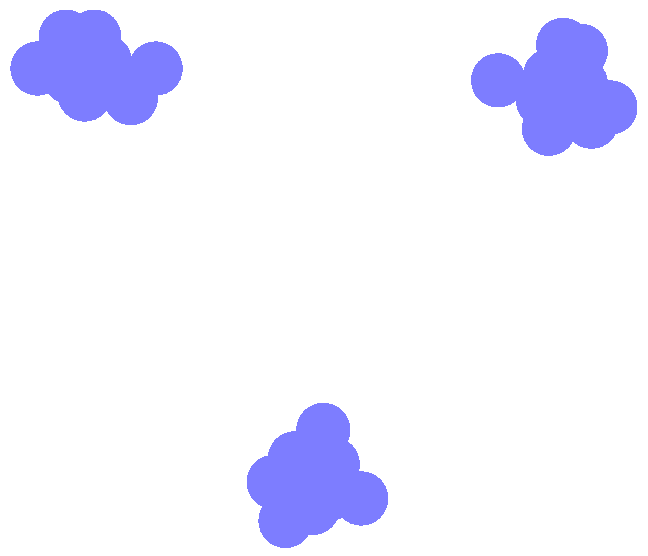
\includegraphics[width=.4\linewidth]{gfx/three_clusters_fat.pdf}
    \caption{$\widehat{X}_\varepsilon$}
    \label{fig:clusters_fat}
  \end{center}
\end{figure}

Allora possiamo possiamo calcolare il numero di componenti connesse di $\widehat{X}_\varepsilon$, o equivalentemente la dimensione del gruppo di omologia $H_{0}(\widehat{X}_\varepsilon;k)$, dove $k$ è un campo. L'osservazione che $X$ è composto essenzialmente da tre componenti è espressa dal fatto che
\begin{equation*}
  \mathrm{dim}_k(H_{0}(\widehat{X}_\varepsilon;k))=3
\end{equation*}
per un intervallo notevole di valori di $\varepsilon$, e da un certo $\overline{\varepsilon}$ in poi diventa~1.

Ovviamente, non è necessario parlare di dimensione del gruppo di omologia $H_{0}$ per discutere del numero di componenti connesse. Tuttavia, se consideriamo l'insieme di dati $X$ come in \cref{fig:circle}, possiamo chiederci come formalizzare l'intuizione che essi sono disposti in forma circolare.

\begin{figure}[h]
  \begin{center}
    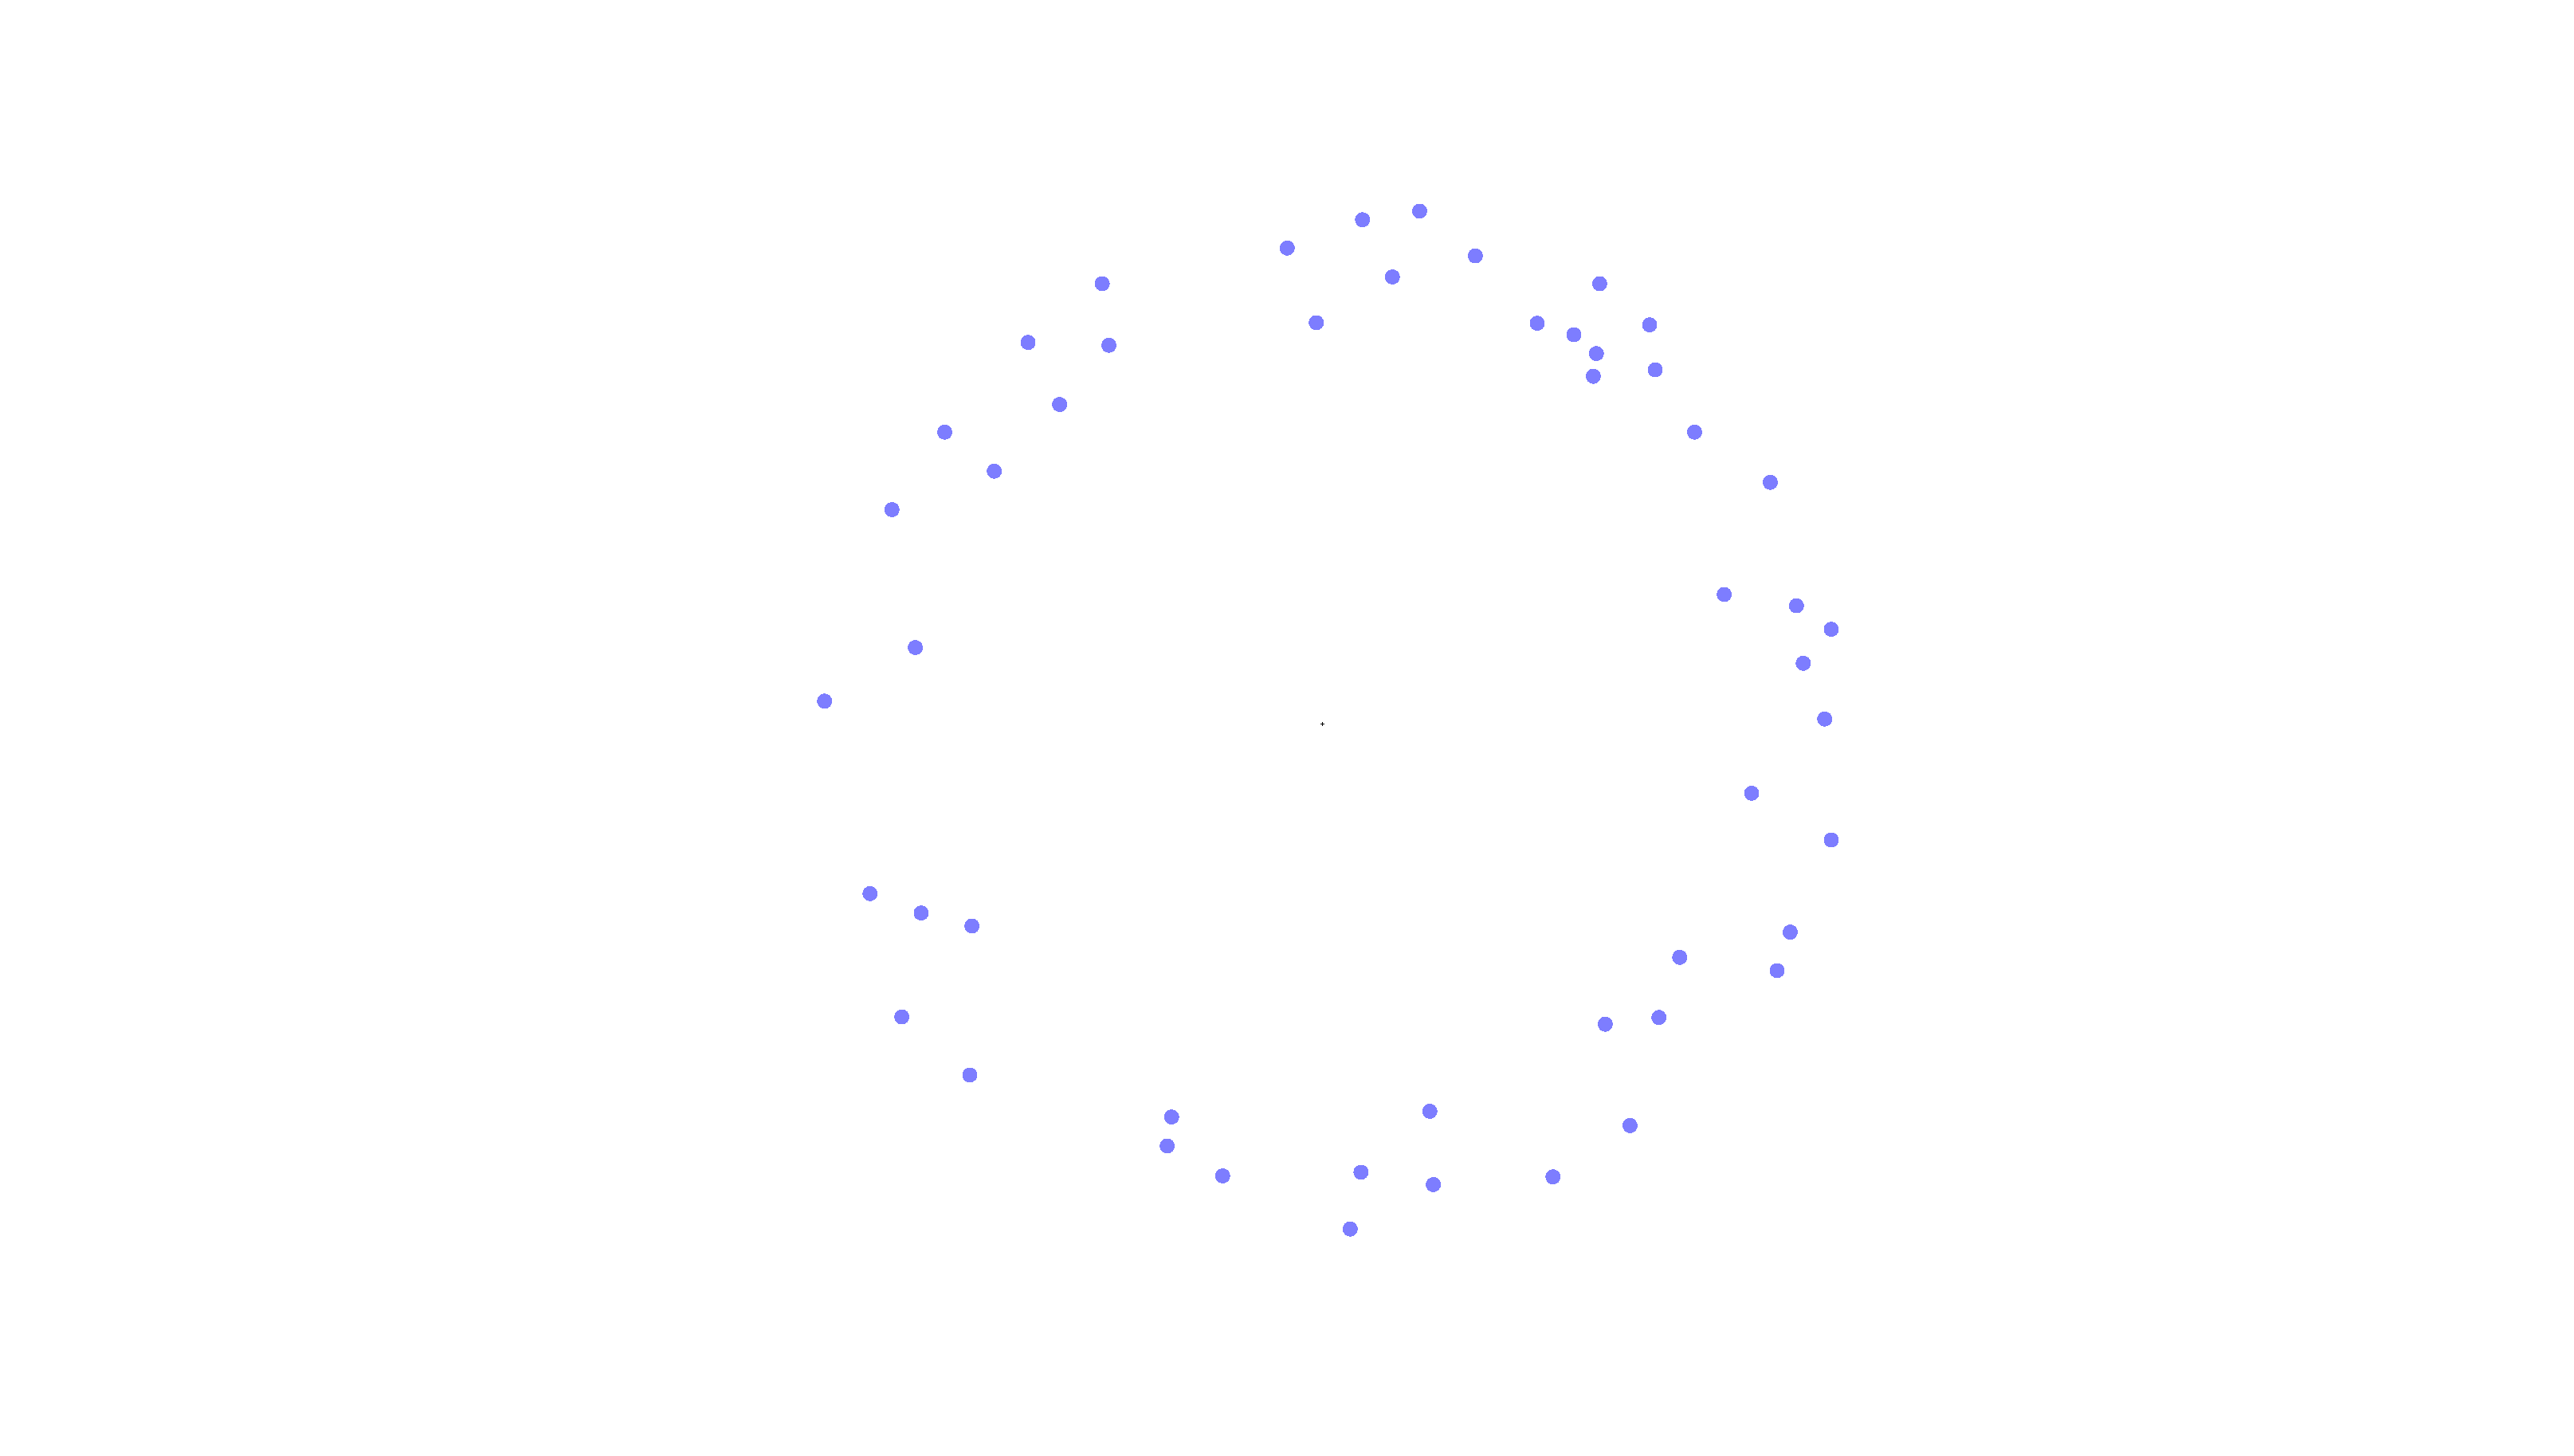
\includegraphics[width=\linewidth]{gfx/statistical_circle.pdf}
    \caption{Campionamento da una corona circolare}
    \label{fig:circle}
  \end{center}
\end{figure}

Ancora una volta possiamo considerare l'insieme $\widehat{X}_\varepsilon$ per diversi valori di $\varepsilon$ come in \cref{fig:circlecomparison} e considerare stavolta il gruppo di omologia $H_{1}(\widehat{X}_\varepsilon;k)$.

\begin{figure}[h]
  \begin{center}
    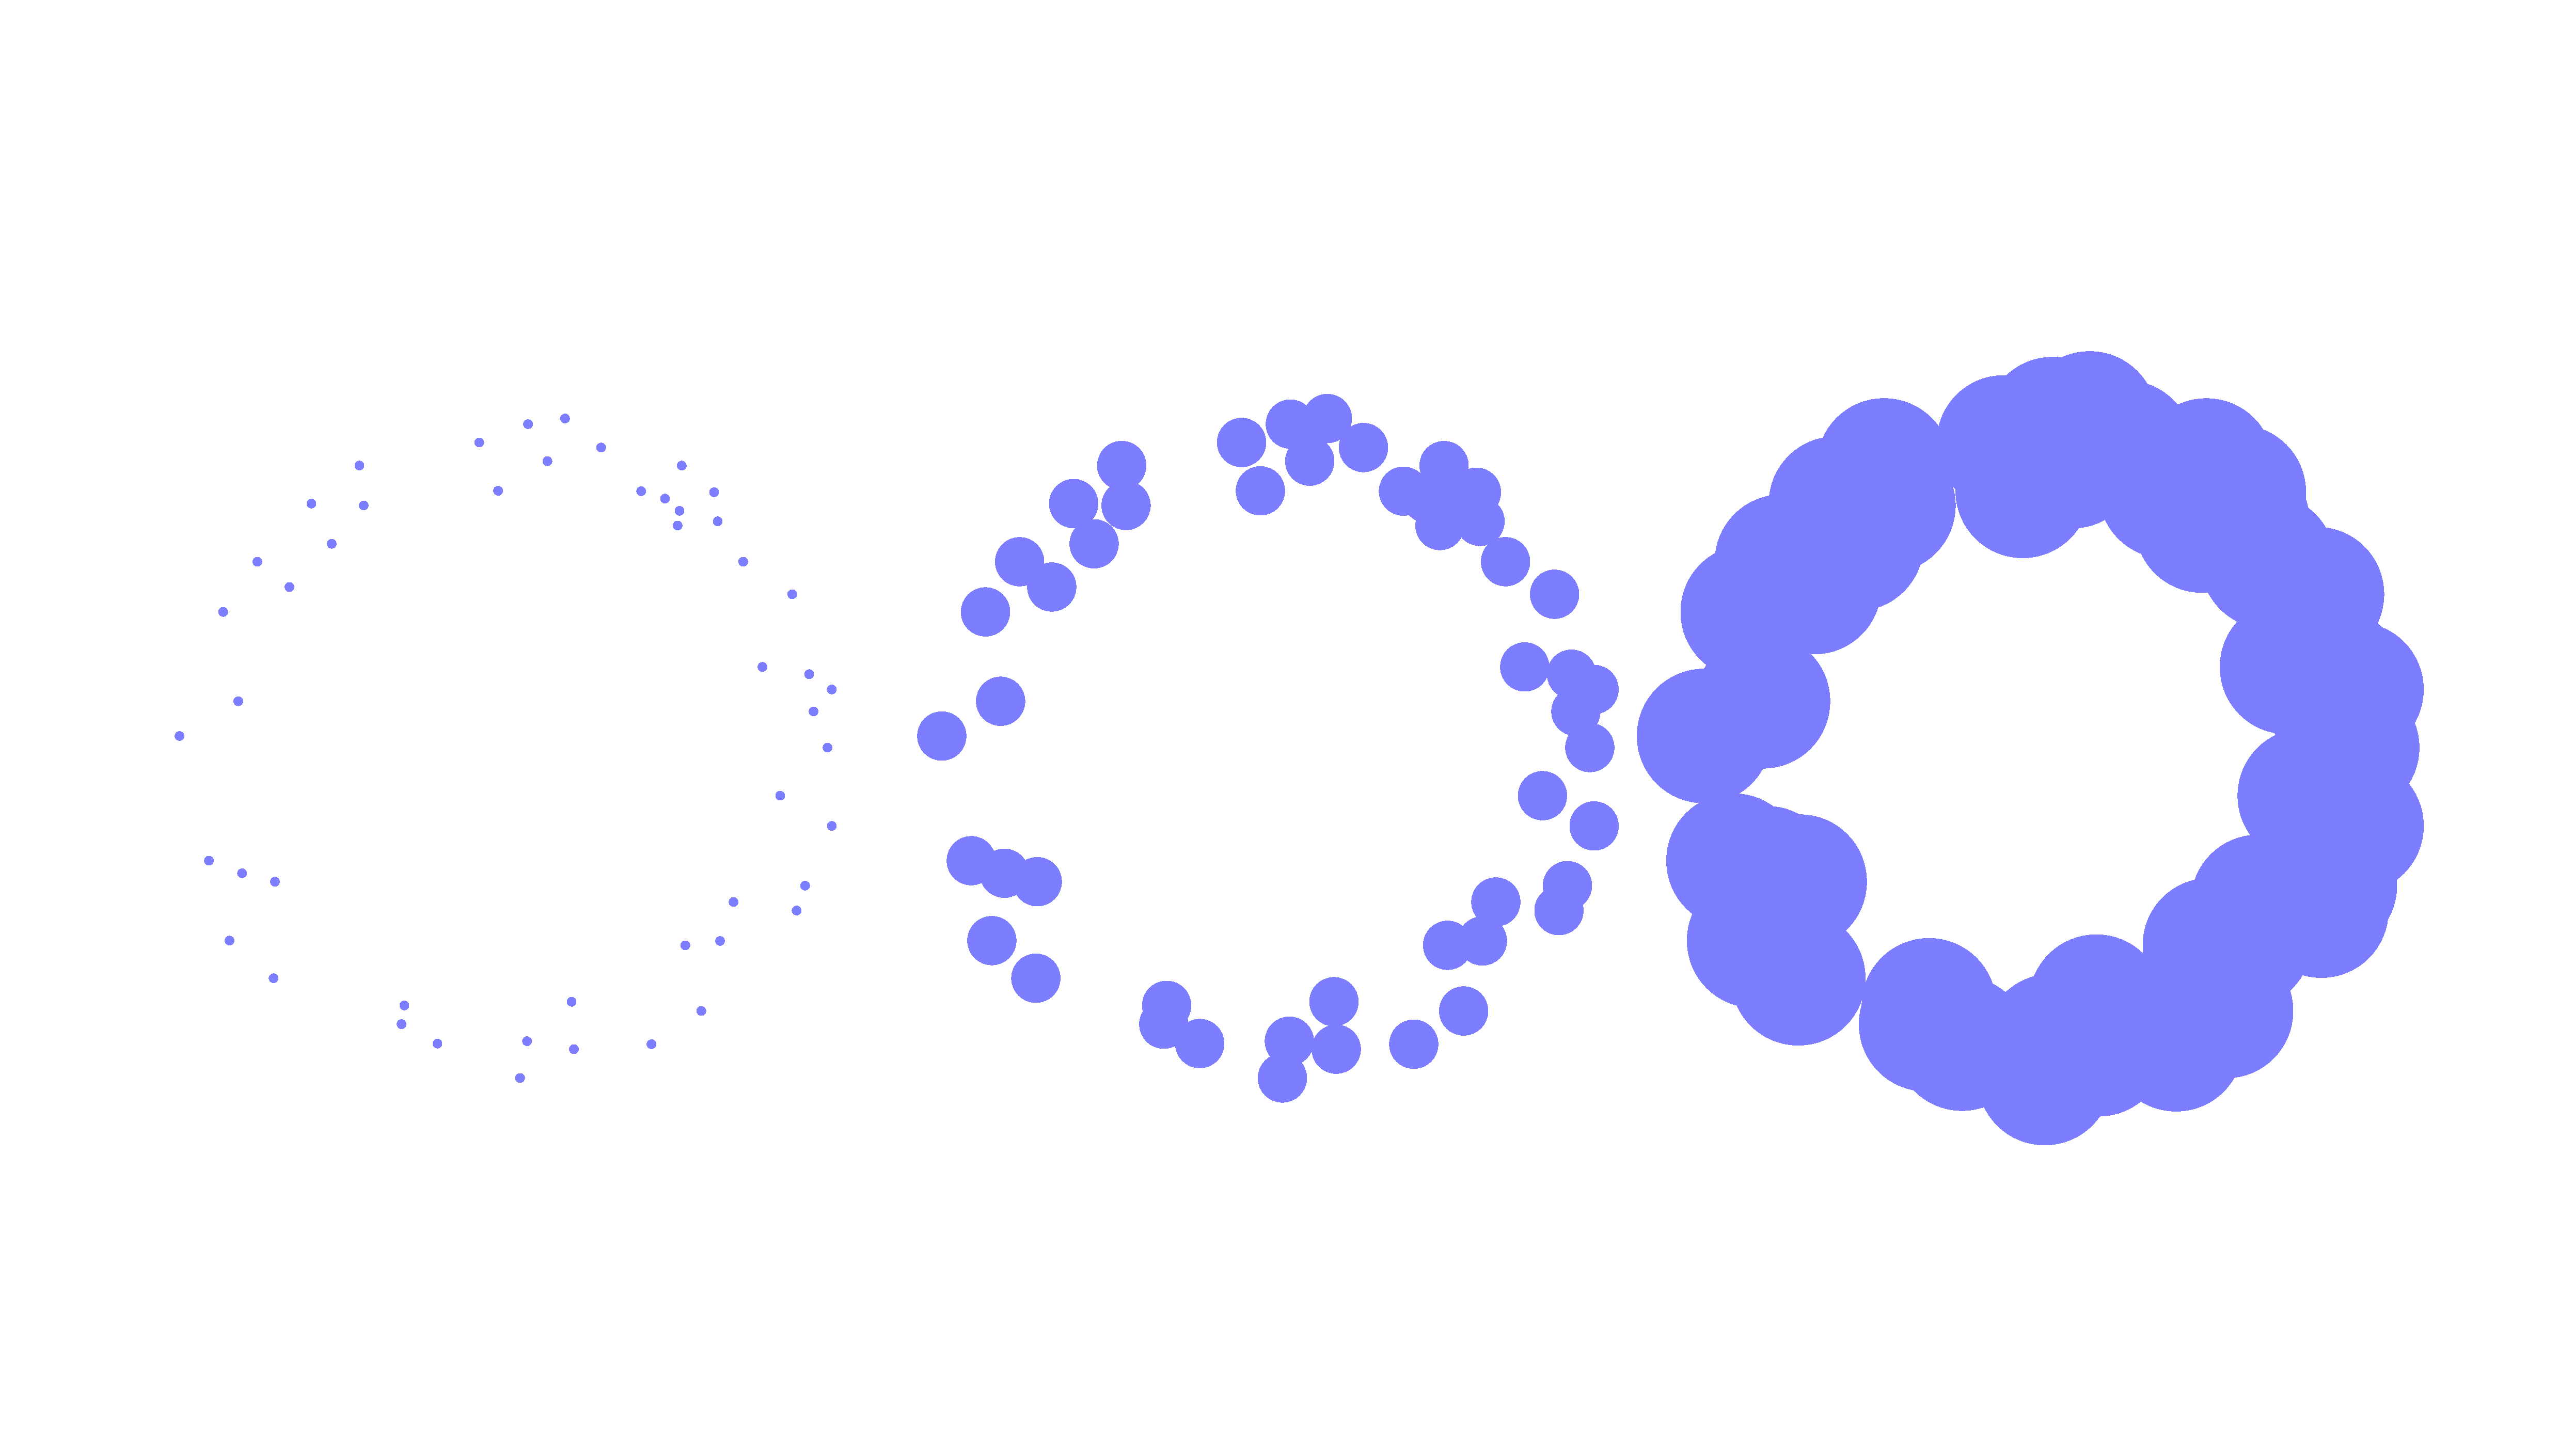
\includegraphics[width=.7\paperwidth]{gfx/statistical_circle_comparison.pdf}
    \caption{$\widehat{X}_\varepsilon$ al variare di $\varepsilon$}
    \label{fig:circlecomparison}
  \end{center}
\end{figure}

La dimensione di $H_1(\widehat{X}_\varepsilon;k)$ varia fino a stabilizzarsi su 1. Questo ci dice che c'è essenzialmente un buco 1-dimensionale nei dati.

Possiamo anche osservare variazioni di struttura al variare della scala di riferimento. Ad esempio, in \cref{fig:moreclusters} possiamo vedere che i tre cluster sulla sinistra collassano in un unico cluster se condiseriamo $\widehat{X}_\varepsilon$ per $\varepsilon \gtrsim e_2/2$.

\begin{figure}[h]
  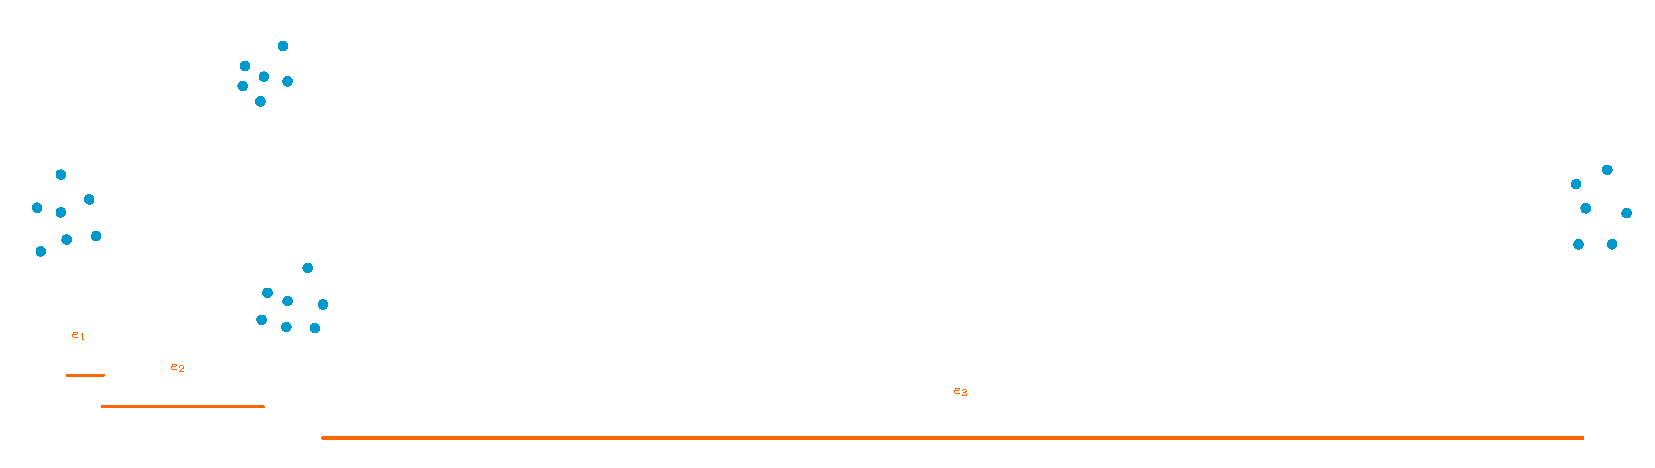
\includegraphics[width=.7\paperwidth]{gfx/more_clusters.pdf}
  \caption{Cluster su scale diverse}
  \label{fig:moreclusters}
\end{figure}

Per visualizzare l'andamento di $dim_k(\widehat{X}_\varepsilon)$ al variare di $\varepsilon$ usiamo un tipo di grafico chiamato \emph{persistence barcode}: per ogni \emph{feature} presente nei dati, disegnamo un segmento orizzontale lungo quanto l'intervallo di lunghezze di $\varepsilon$ in cui la feature persiste, come in \cref{fig:moreclusterbarcode}.

\begin{figure}[h]
  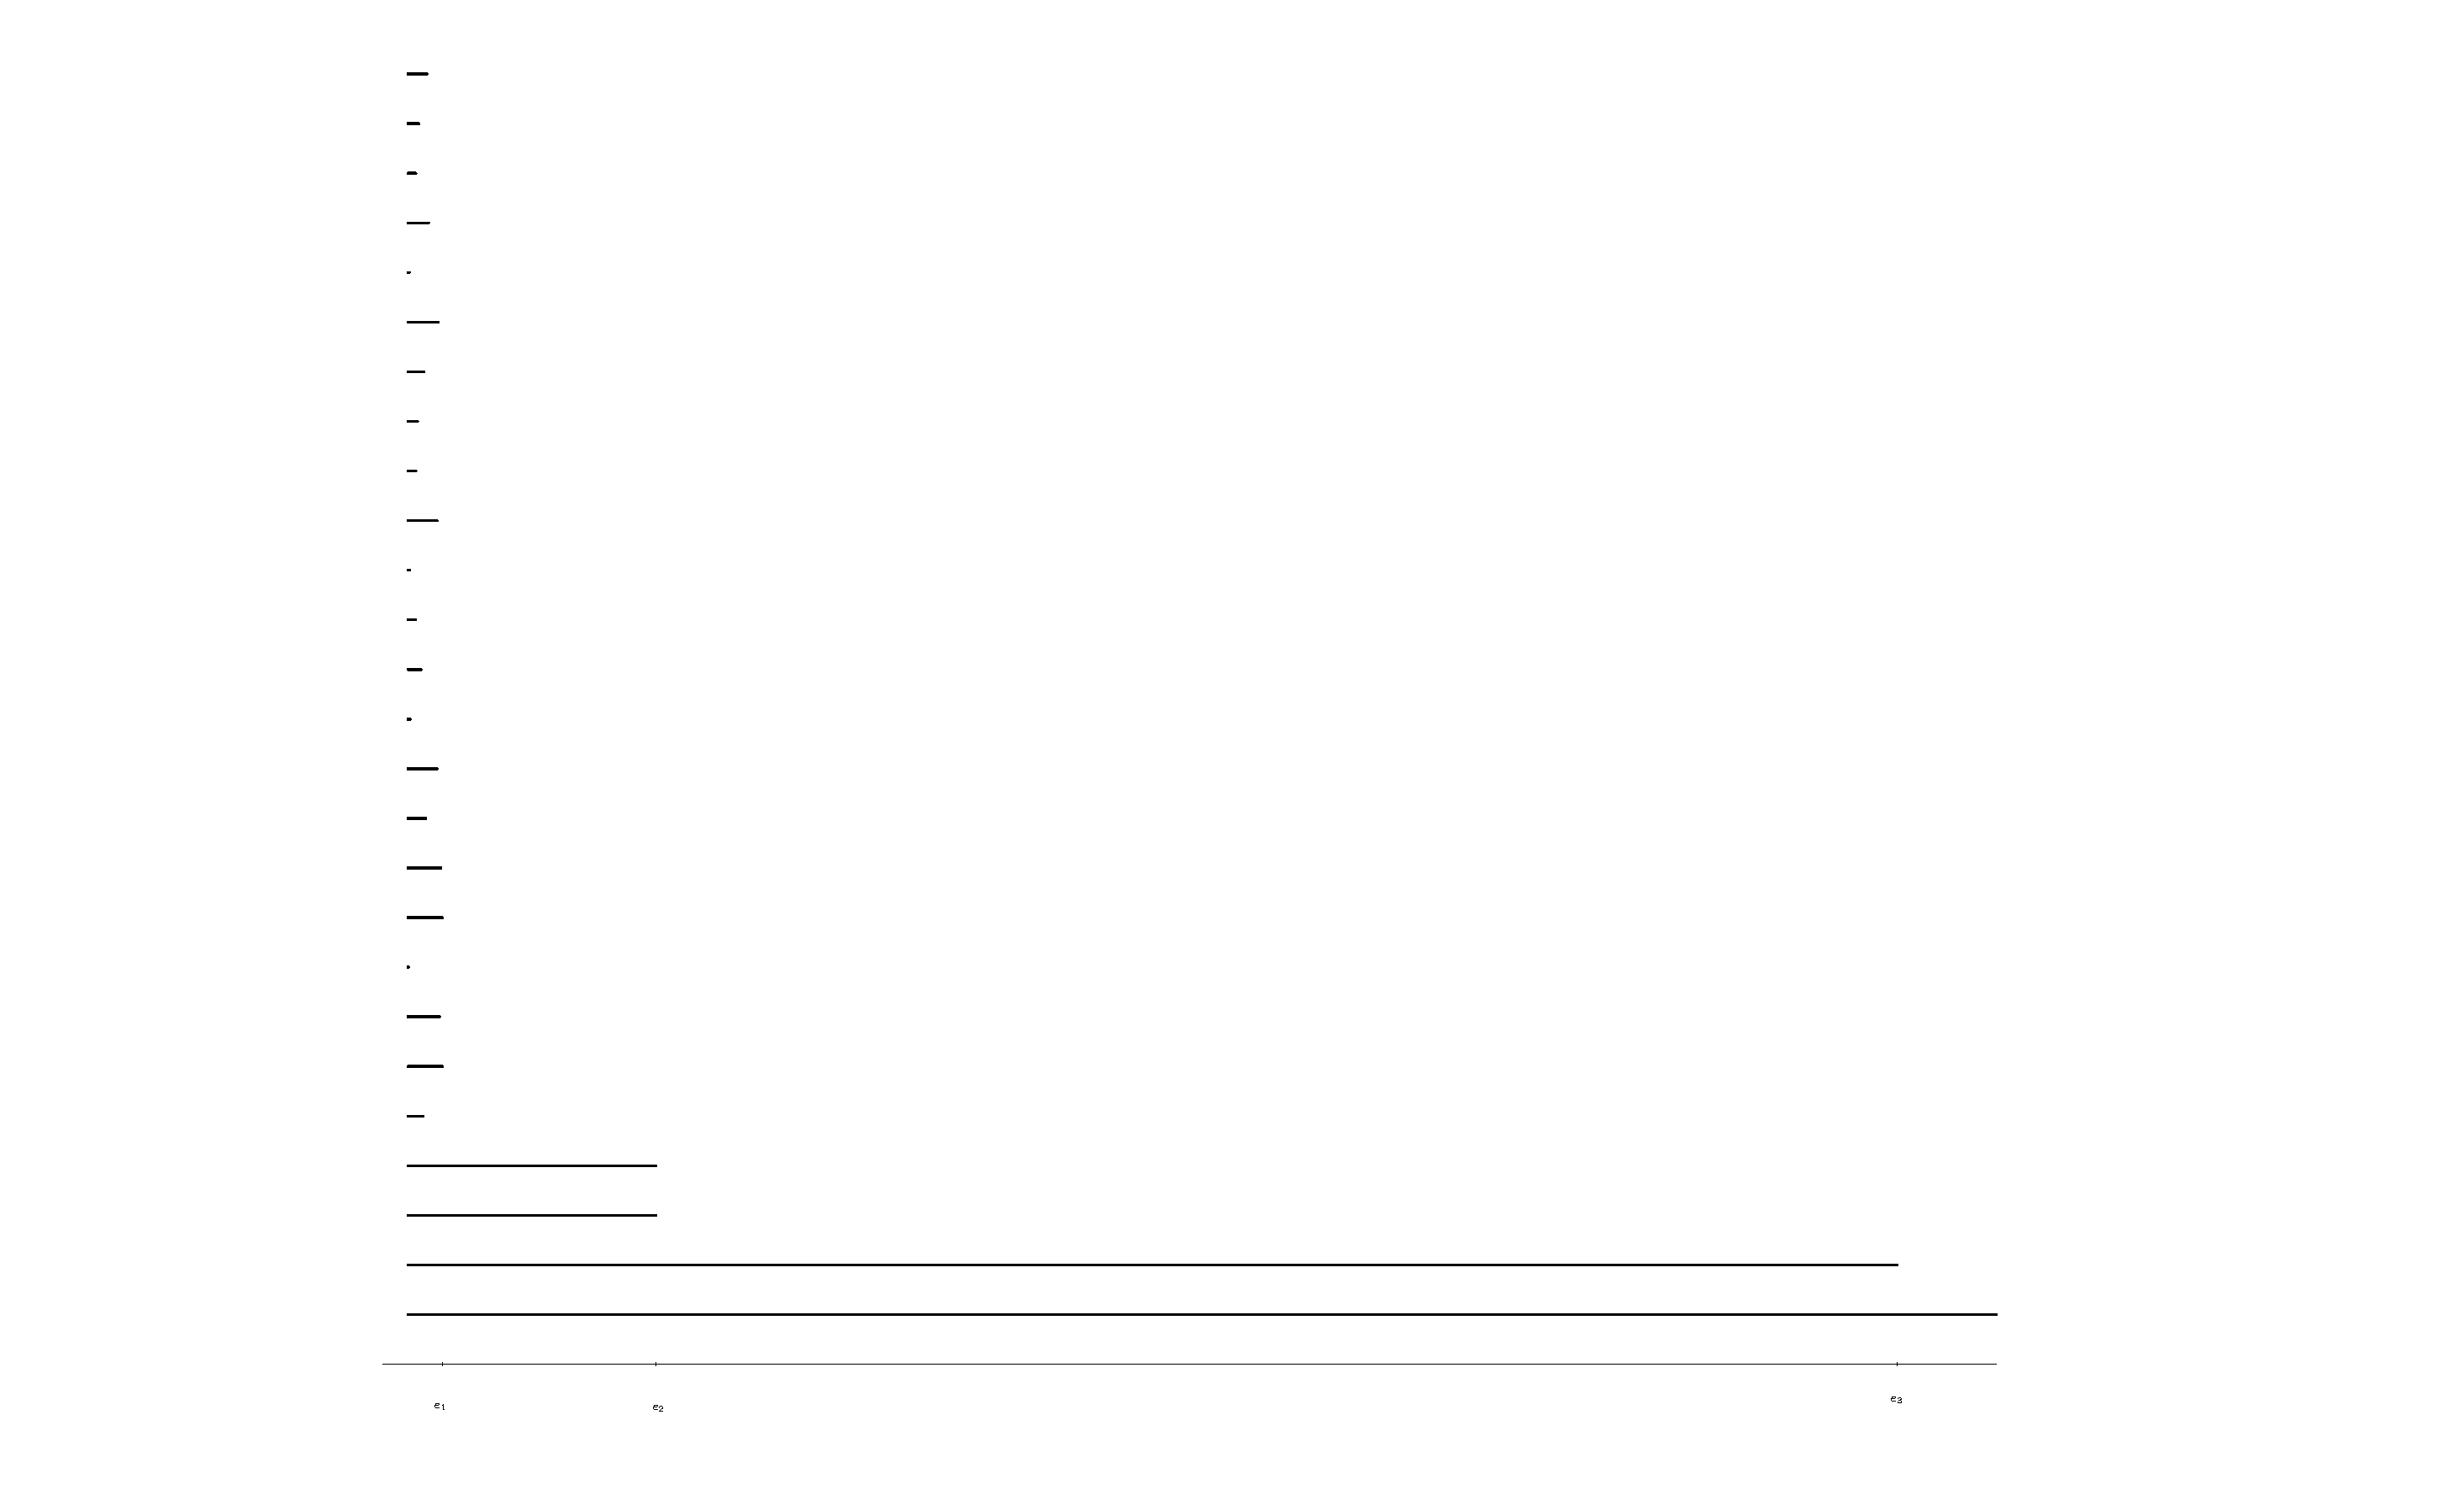
\includegraphics[width=.7\paperwidth]{gfx/more_clusters_barcodes.pdf}
  \caption{Un esempio di persistence barcode}
  \label{fig:moreclusterbarcode}
\end{figure}

Il grafico fa interpretato nel seguente modo: all'inizio vi sono 26 punti distinti, al crescere di $\varepsilon$ questi punti vengono uniti ad altri e quindi il numero si riduce, finché per $\varepsilon \gtrsim e_1/2$ restano essenzialmente 4 cluster, da $e_2/2$ ne restano solo due e da $e_3/2$ il gruppo di omologia $H_0(\widehat{X}_\varepsilon;k)$ diventa banale. (NMDC: aggiusta il grafico del barcode)

Possiamo sempre usare questa rappresentazione grazie alla decomposizione dei persistence barcodes garantita dal teorema (NMDC: aggiungere riferimento).

Un altro aspetto che l'omologia persistente cattura è la relazione fra i gruppi di omologia nelle diverse scale, in particolare $H_*(\widehat{X}_\varepsilon;k)$ è funtoriale rispetto all'ordine di $(\R,\leq)$, cioé se $\varepsilon_1 \leq \varepsilon_2$ allora c'è una mappa $H_*(\widehat{X}_{\varepsilon_1};k)\to H_*(\widehat{X}_{\varepsilon_2};k)$ e se $\varepsilon_1\leq\varepsilon_2\leq\varepsilon_3$, allora la mappa associata a $\varepsilon_1\leq\varepsilon_3$ è uguale alla composizione delle due mappe associate a $\varepsilon_1\leq\varepsilon_2$ e $\varepsilon_2\leq\varepsilon_3$.

Questo ci consente di catturare proprietà come quelle che si osservano in \cref{fig:doublecircle}.

\begin{figure}[ht]
  \begin{center}
    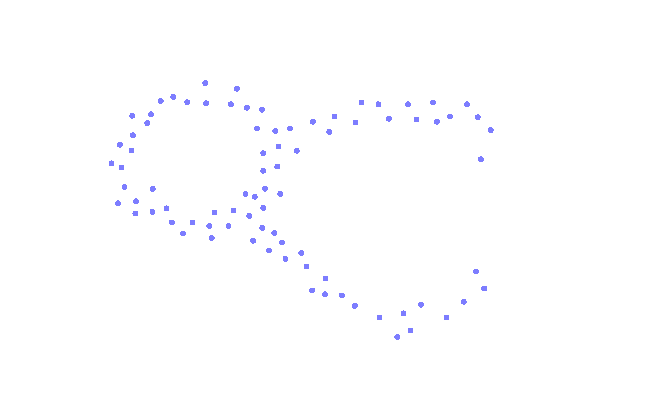
\includegraphics{gfx/double_circle_small.pdf}
    \caption{Un doppio anello}
    \label{fig:doublecircle}
  \end{center}
\end{figure}

In \cref{fig:doublecirclecomparison} osserviamo che al variare di $\varepsilon$ la dimensione di $H_1(\widehat{X}_\varepsilon;k)$ resta 1, tuttavia è chiaro che i due anelli sono due proprietà distinte dei dati. Questa distinzione non è racchiusa nel gruppo di omologia $H_1$, mentre la si vede dal fatto che la mappa
\begin{equation*}
H_1(\widehat{X}_{\varepsilon_1};k)\xto{0}H_1(\widehat{X}_{\varepsilon_2};k)
\end{equation*}
associata a $\varepsilon_1\leq\varepsilon_2$ è il morfismo nullo. Questo ci dice che non ci sono relazioni fra i due gruppi di omologia.

\begin{figure}[ht]
  \begin{center}
    \begin{subfigure}[b]{.4\textwidth}
      
\includegraphics[width=\textwidth]{gfx/double_circle_medium.pdf}
      \caption{$\widehat{X}_{\varepsilon_1}$}
    \end{subfigure}
    \begin{subfigure}[b]{.4\textwidth}
      
\includegraphics[width=\textwidth]{gfx/double_circle_fat.pdf}
      \caption{$\widehat{X}_{\varepsilon_2}$}
    \end{subfigure}
    \caption{Variazione delle proprietà di $\widehat{X}_\varepsilon$}  \label{fig:doublecirclecomparison}
  \end{center}
\end{figure}

(NMDC:dire qualcosa sull'algoritmo Mapper?)

Nel resto del capitolo ci occuperemo di costruire l'omologia persistente, con attenzione all'aspetto computazionale.

\clearpage

\section{Omologia simpliciale}

\begin{sloppypar}
  Fissato un campo $k$, ad ogni spazio topologico possiamo associare una successione di $k$-spazi vettoriali $H_i(X;k)$ detti \emph{gruppi di omologia}. Per la precisione si tratta di una successione di funtori ${H_*(-;k):\Top \to \Vectk}$. Nel resto della sezione ci occuperemo di definire in modo operativo questi gruppi.
\end{sloppypar}

Esistono diversi modi di calcolare i gruppi di omologia. Il più generale e potente è l'omologia singolare, tuttavia questa risulta scomoda da usare in pratica perché richiede di lavorare con quozienti di spazi vettoriali di dimensione più che numerabile. Per aggirare il problema definiremo soltanto l'omologia simpliciale.

In virtù degli assiomi di Eilenberg-Steenrod \cite{Eilenberg1945, Eilenberg} le due definizioni sono equivalenti (almeno per gli spazi che andremo a considerare). Per una trattazione più dettagliata si vedano \cite{Hatcher2015} o \cite{Rotman1988}.

Si procederà associando all'insieme di dati $X$ uno spazio topologico (detto complesso simpliciale) per ogni parametro $\varepsilon \in \R^+$ e si definirà l'omologia solo per questi particolari spazi topologici.

Gli spazi $\widehat{X}_\varepsilon$ usati nell'introduzione, sebbene comodi per introdurre un'idea intuitiva di persistenza, non sono l'ambiente naturale in cui lavorare, quindi non verranno più usati nella trattazione formale. Si osservi, però, che l'omologia di $\widehat{X}_\varepsilon$ è equivalente all'omologia del complesso simpliciale di \v{C}ech di parametro $\varepsilon$ associato a $X$. Per questioni di comodità, tuttavia, noi lavoreremo principalmente con il complesso di Vietoris-Rips.

\subsection{Complessi simpliciali}

\begin{sloppypar}
  I complessi simpliciali sono particolari spazi topologici che hanno una descrizione combinatorica. Dato un insieme di punti ${S=\{s_0,\dots,s_n\}}$ in $\R^k$ diremo che sono in posizione generale se non sono contenuti in nessun sottospazio affine di dimensione minore di $n$. Se $S$ è in posizione generale, il suo inviluppo convesso $\sigma(S)$ è detto \emph{($n$-)simplesso generato da $S$}. I punti $s_i$ di $S$ si chiamano \emph{vertici} di $\sigma(S)$. Se $\emptyset\neq T$ è un sottinsieme di $S$, $\sigma(T)$ è detto \emph{faccia} di $\sigma(S)$.
\end{sloppypar}

Con questi ingredienti possiamo dare la seguente
\begin{defn}
Un \emph{complesso simpliciale} (finito) $K$ è una famiglia finita di simplessi in uno spazio euclideo tali che:
\begin{enumerate}
  \item Se $\sigma\in K$ e $\tau$ è una faccia di $\sigma$, allora $\tau \in K$.
  \item Se $\sigma,\tau\in K$, allora il simplesso $\sigma\cap\tau$ è una faccia sia di $\sigma$ sia di $\tau$.
\end{enumerate}
\end{defn}

\`E chiaro che un complesso simpliciale è determinato essenzialmente da proprietà combinatoriche dell'insieme dei suoi vertici, che motiva la seguente costruzione astratta.

\begin{defn}
  Un \emph{complesso simpliciale astratto} $X$ è il dato della coppia $(V(X), \Sigma(X))$, dove $V(X)$ è un insieme finito, i cui elementi sono i \emph{vertici} di $X$, e $\Sigma(X)$ è una famiglia di sottinsiemi non vuoti di $V(X)$, i cui elementi sono detti \emph{simplessi} di $X$, tale che:
  \begin{enumerate}
    \item se $v\in V(x)$ allora $\{v\}\in\Sigma(X)$, e
    \item se $\sigma \in \Sigma(X)$ e $\emptyset\neq\tau\subseteq\sigma$, allora $\tau\in\Sigma(X)$.
  \end{enumerate}
\end{defn}

\begin{rmk}
  Ogni complesso simpliciale $K$ determina un complesso simpliciale astratto $\widehat{K}$ tale che $V(\widehat{K})$ è l'insieme dei vertici dei simplessi di $K$ e un sottinsieme di $V(\widehat{K})$ è in $\Sigma(\widehat{K})$ se e solo se è l'insieme dei vertici di un simplesso di $K$.
\end{rmk}

Possiamo anche definire i morfismi $f:X\to Y$ fra complessi simpliciali astratti come le mappe $f_V:V(X)\to V(Y)$ fra i sottostanti insiemi di vertici e tali che $f_V(\sigma)\in \Sigma(Y)$ per ogni $\sigma \in \Sigma(X)$.

(NMDC: inserire qualche disegno, eventualmente un riferimento a qualche testo sugli oggetti simpliciali)

Ad ogni complesso simpliciale astratto $X$ si può associare un complesso simpliciale $|X|$ detto la \emph{realizzazione geometrica} di $X$ (NMDC: aggiungere un riferimento) e tale che i morfismi $f:X\to Y$ siano mandati in mappe continue $|f|:|X|\to |Y|$ in maniera funtoriale, cioé $|g\circ f|=|g|\circ |f|$. Inoltre, ogni complesso simpliciale $K$ è omeomorfo alla realizzazione geometrica del complesso simpliciale astratto $\widehat{K}$ ad esso associato.

\subsection{Omologia simpliciale}

Ora definiremo i gruppi di omologia associati a un complesso simpliciale astratto.

\begin{defn}
  Sia $k$ un gruppo o un campo o un anello e
  sia $X=(V(X),\Sigma(X))$ un complesso simpliciale astratto, insieme con un ordine totale sull'insieme $V(X)$. Il gruppo dei \emph{$q$-cicli} di $X$ su $k$ è il $k$-modulo $C_q(X)$ generato dagli elementi
  \begin{itemize}
    \item $[v_0,\dots, v_q]$ con $v_0,\dots, v_q\in V(X)$ e tali che $\{v_0,\dots,v_q\}\in\Sigma(X)$
  \end{itemize}
  modulo le seguenti relazioni:
  \begin{enumerate}
    \item $[v_0,\dots,v_q]=0$ se $v_i = v_j$ per qualche $i\neq j$,
    \item $[v_{\sigma(0)},\dots,v_{\sigma(q)}]=sign(\sigma)[v_0,\dots,v_q]$ per ogni permutazione $\sigma$ di $\{0,\dots,q\}$.
  \end{enumerate}

  Scriveremo $C_*$ per indicare tutti i gruppi dei cicli in tutti i gradi.
\end{defn}

\begin{rmk}
  Nella definizione precedente si è tenuta traccia dell'ordine dei vertici dei complessi simpliciali perché esso è importante ai fini dell'omologia, dunque d'ora in poi consideriamo sempre i complessi simpliciali ordinati.
\end{rmk}

\begin{lemma}\label{lemma:sollcicli}
  Dati due complessi simpliciali astratti $X$ e $Y$ e un morfismo $f$ fra essi, allora $f$ induce un omomorfismo $f_q:C_q(X)\to C_q(Y)$ per ogni $q\in\mathbb{N}$ definito da:
  \begin{align*}
    f_q:C_q(X)\longrightarrow & C_q(Y)\\
    [v_0,\dots,v_q] \mapsto & [f(v_0),\dots,f(v_q)].
  \end{align*}

  Scriveremo $f_*:C_*(X)\to C_*(Y)$ per indicare tutti questi morfismi.
\end{lemma}

\begin{rmk}
  Il motivo per cui il gruppo dei $q$-cicli è stato introdotto mediante generatori e relazioni è che in questo modo è più facile sollevare mappe di complessi simpliciali astratti a omomorfismi fra i gruppi dei cicli. Se avessimo semplicemente definito il gruppo dei $q$-cicli come il $k$-modulo generato da $X_q$ sarebbe stato necessario modificare la definizione di $f_*$ in modo che i cicli mappassero correttamente, perdendo notevolmente in eleganza.
\end{rmk}

\cleardoublepage
%*****************************************
\chapter{Introduzione}\label{ch:introduction}

Negli ultimi anni molte branche della scienza e dell'industria si trovano a produrre e analizzare insiemi di dati sempre più grandi e complessi. Questi Big Data sono difficilmente analizzabili usando tecniche standard a causa di problemi sia tecnici che teorici.

Ad esempio, dover processare grandi quantità di dati complessi può avere facilmente un costo troppo elevato in termini di tempo e memoria rispetto alle possibilità della tecnologia odierna. Vi sono poi problemi che si annidano nell'analisi di dati in elevate dimensioni, in cui bisogna tenere conto di alcune particolarità, come il fatto che la distanza fra due punti smette di essere significativa.

Si può visualizzare questa cosa confrontando l'estrazione casuale di punti dal quadrato in dimensione 2 o dall'ipercubo in dimensione 100: estratti due punti $x$ e $y$ dalla distribuzione uniforme sull'ipercubo unitario in $\R^d$, la distanza fra loro è
\begin{equation*}
  d(x,y) = \sqrt{\sum_{i=1}^d (x_i - y_i)^2},
\end{equation*}
allora per la disuguaglianza di Hoeffding la distribuzione di $d(x,y)$ è concentrata attorno al valore medio per dimensioni $d$ elevate. In \cref{fig:pointdistance} si può vedere la differenza: i due grafici mostrano l'andamento della distanza di un punto casuale dell'ipercubo da altri 100 punti casuali per $d=2$ e $d=100$. Si può notare come all'aumentare della dimensione i valori si schiacciano attorno al valor medio.

\begin{figure}[ht]
  \begin{center}
    \begin{subfigure}[b]{.4\textwidth}
      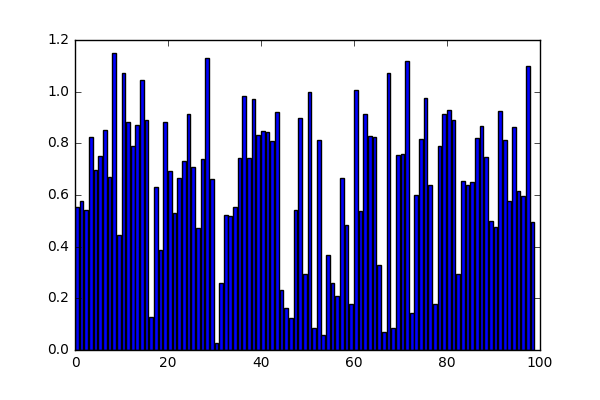
\includegraphics[width=\textwidth]{gfx/pltpoints2d.png}
      \caption{$d=2$}
    \end{subfigure}
    \begin{subfigure}[b]{.4\textwidth}
      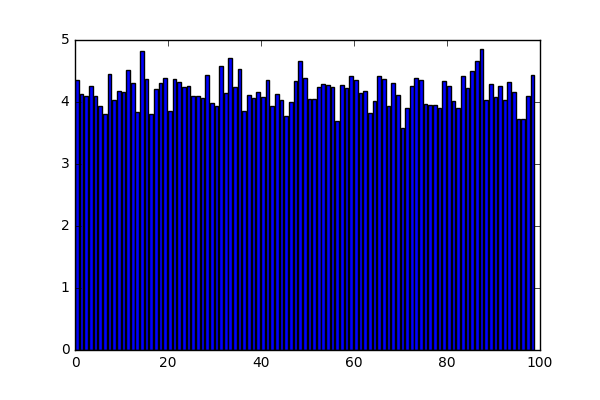
\includegraphics[width=\textwidth]{gfx/pltpoints100d.png}
      \caption{$d=100$}
    \end{subfigure}
    \caption{Distanza fra punti casuali nell'ipercubo}  \label{fig:pointdistance}
  \end{center}
\end{figure}

Ci interessa quindi sviluppare tecniche in grado di rivelare informazioni in spazi metrici di dimensione possibilmente elevata, in particolare vorremmo poter riassumere in un numero finito (piccolo) di variabili l'informazione che ci serve.

Utilizzeremo tecniche di topologia algebrica, e le informazioni che queste ci consentiranno di catturare riguardano la \emph{forma} dei dati. In dimensioni elevate è difficile visualizzare un insieme di punti e quindi comprendere se questo abbia una forma interessante, tuttavia utilizzando la topologia è possibile produrre una rappresentazione sintetica di uno spazio complesso mediante una quantità finita di informazioni, e tale che calcolando opportuni invarianti di questa rappresentazione si ricavino informazioni sulla \emph{forma} dello spazio. La topologia consente anche di esprimere mediante quantità precise cosa intendiamo per \emph{forma}.

Prendendo ad esempio la corona circolare in \cref{fig:annulus}, la proprietà che vogliamo essere in grado di catturare è il fatto che essa contiene essenzialmente un solo loop non banale a meno di omotopia, o in maniera equivalente potremmo dire che ha un unico foro.

\begin{figure}[ht]
  \begin{center}
    
\includegraphics[width=.5\textwidth]{gfx/annulus.pdf}
    \caption{Corona circolare}  \label{fig:annulus}
  \end{center}
\end{figure}

Vorremmo anche essere in grado di rappresentare sinteticamente uno spazio mediante simplessi, conservando quanta più informazione possibile sulla sua forma. Ad esempio passando dalla circonferenza al quadrato in \cref{fig:circsquare} perdiamo informazioni sulla curvatura, tuttavia le proprietà topologiche sono invariate.

\begin{figure}[ht]
  \begin{center}
    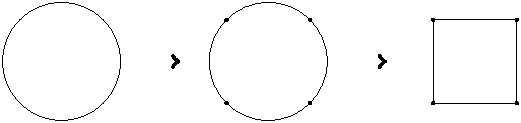
\includegraphics[width=.7\textwidth]{gfx/circsquare.pdf}
    \caption{Rappresentazione di una circonferenza}  \label{fig:circsquare}
  \end{center}
\end{figure}

Nel tipo di applicazione che ci interessa, tuttavia, l'oggetto di studio non è una varietà come nei casi precedenti, ma una nube di punti, cioé un sottinsieme finito di $\R^d$ o più in generale uno spazio metrico finito $X=\{x_1,\dots,x_n\}$. Anche in questo caso lo spazio può esibire una forma interessante, ad esempio in \cref{fig2:clusters} i dati si dispongono chiaramente in tre gruppi, mentre in \cref{fig2:circle} hanno chiaramente una forma circolare.

\begin{figure}[ht]
  \begin{center}
    
\includegraphics[width=.4\linewidth]{gfx/three_clusters_small.pdf}
    \caption{Dati divisi in più cluster}
    \label{fig2:clusters}
  \end{center}
\end{figure}

\begin{figure}[ht]
  \begin{center}
    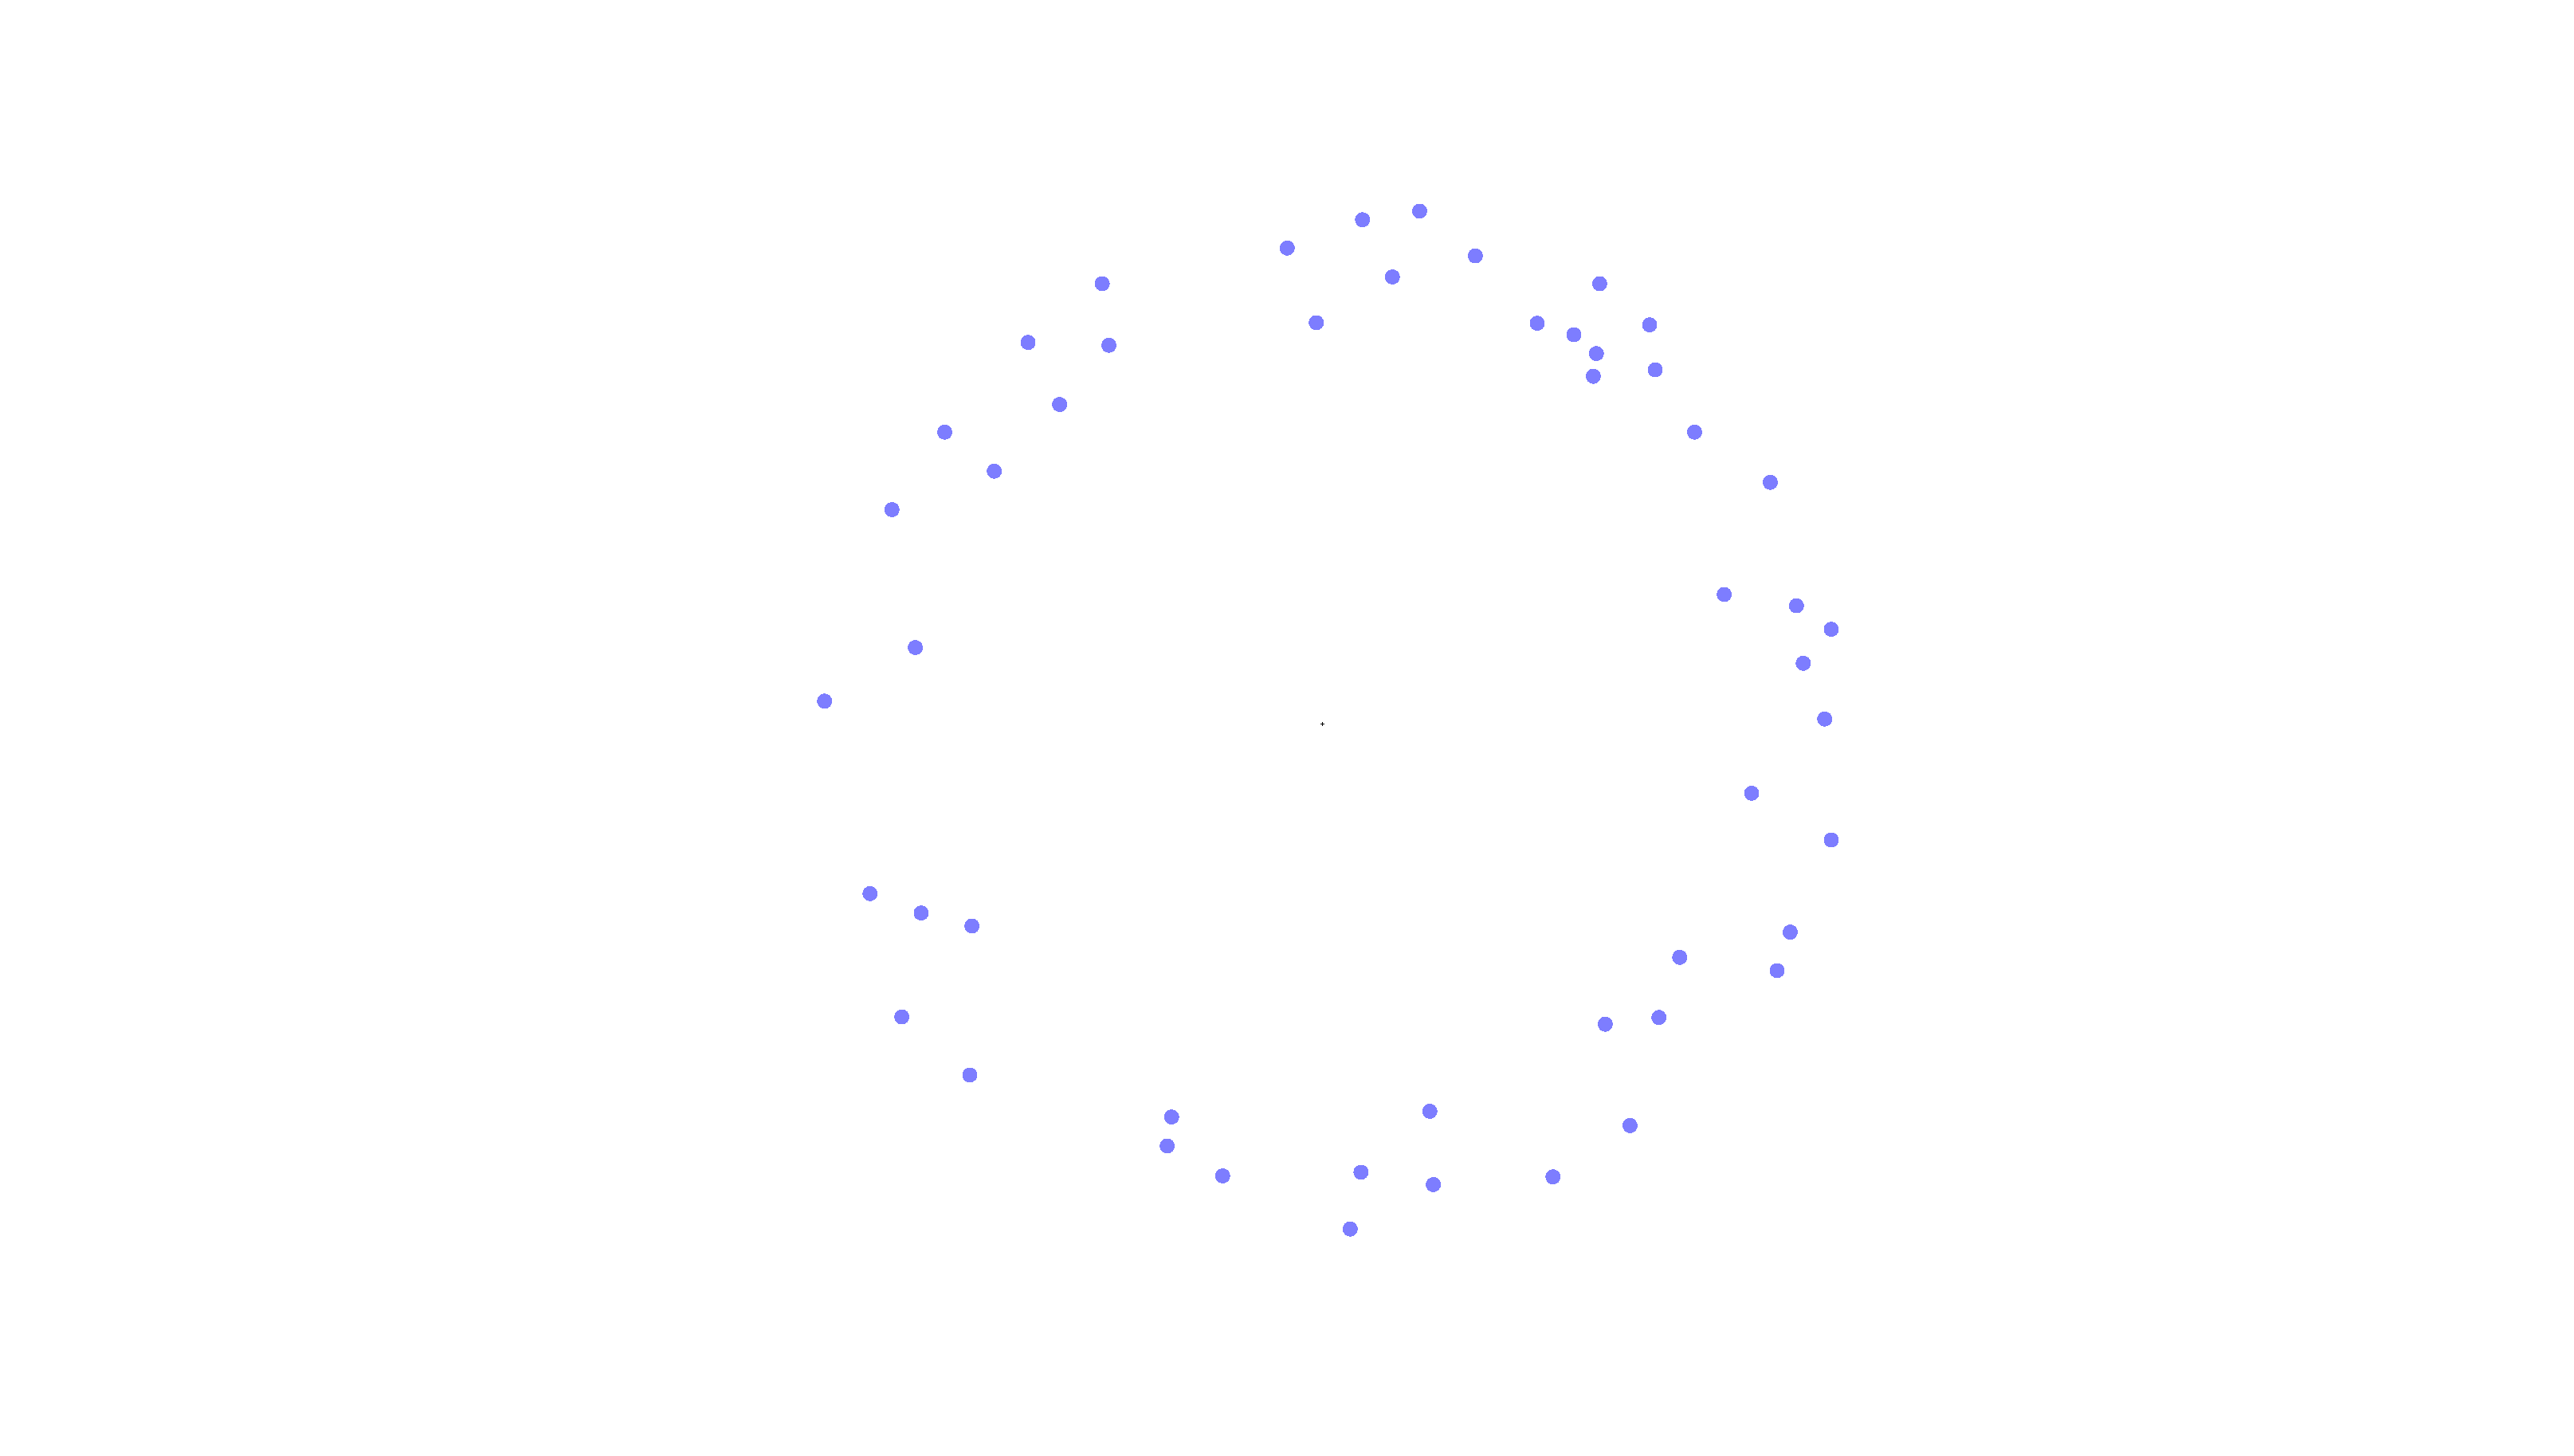
\includegraphics[width=\linewidth]{gfx/statistical_circle.pdf}
    \caption{Campionamento da una corona circolare}
    \label{fig2:circle}
  \end{center}
\end{figure}

Come si possono esprimere queste osservazioni mediante tecniche algebriche? Se i nostri dati sono collezionati nell'insieme finito $X=\{x_1,\dots,x_n\}\subseteq \R^d$, possiamo considerare
\begin{equation*}
  \widehat{X}_\varepsilon = \bigcup_{x\in X} B_\varepsilon(x)
\end{equation*}
dove $B_\varepsilon(x)$ è la palla di raggio $\varepsilon$ e centro $x$. Allora per qualche opportuno $\varepsilon >0$ l'insieme $\widehat{X}_\varepsilon$ associato alla \cref{fig2:clusters} diventa del tipo raffigurato in \cref{fig2:clusters_fat}.

\begin{figure}[h]
  \begin{center}
    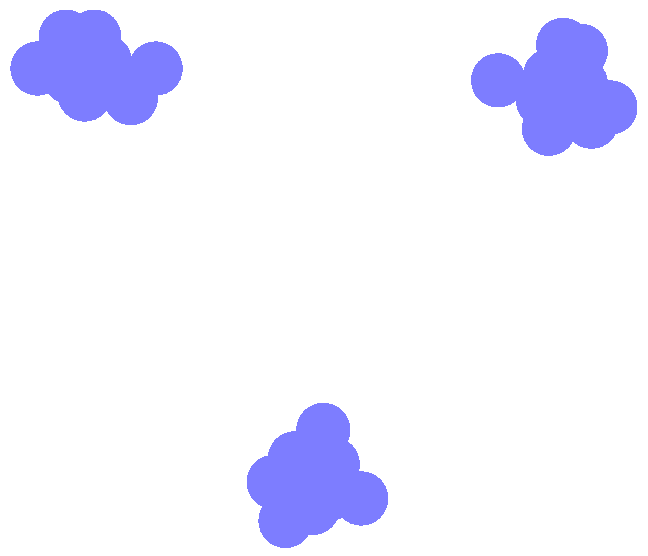
\includegraphics[width=.4\linewidth]{gfx/three_clusters_fat.pdf}
    \caption{$\widehat{X}_\varepsilon$}
    \label{fig2:clusters_fat}
  \end{center}
\end{figure}

Analogamente al variare di $\varepsilon$ vediamo gli spazi mostrati in \cref{fig2:circlecomparison}.

\begin{figure}[h]
  \begin{center}
    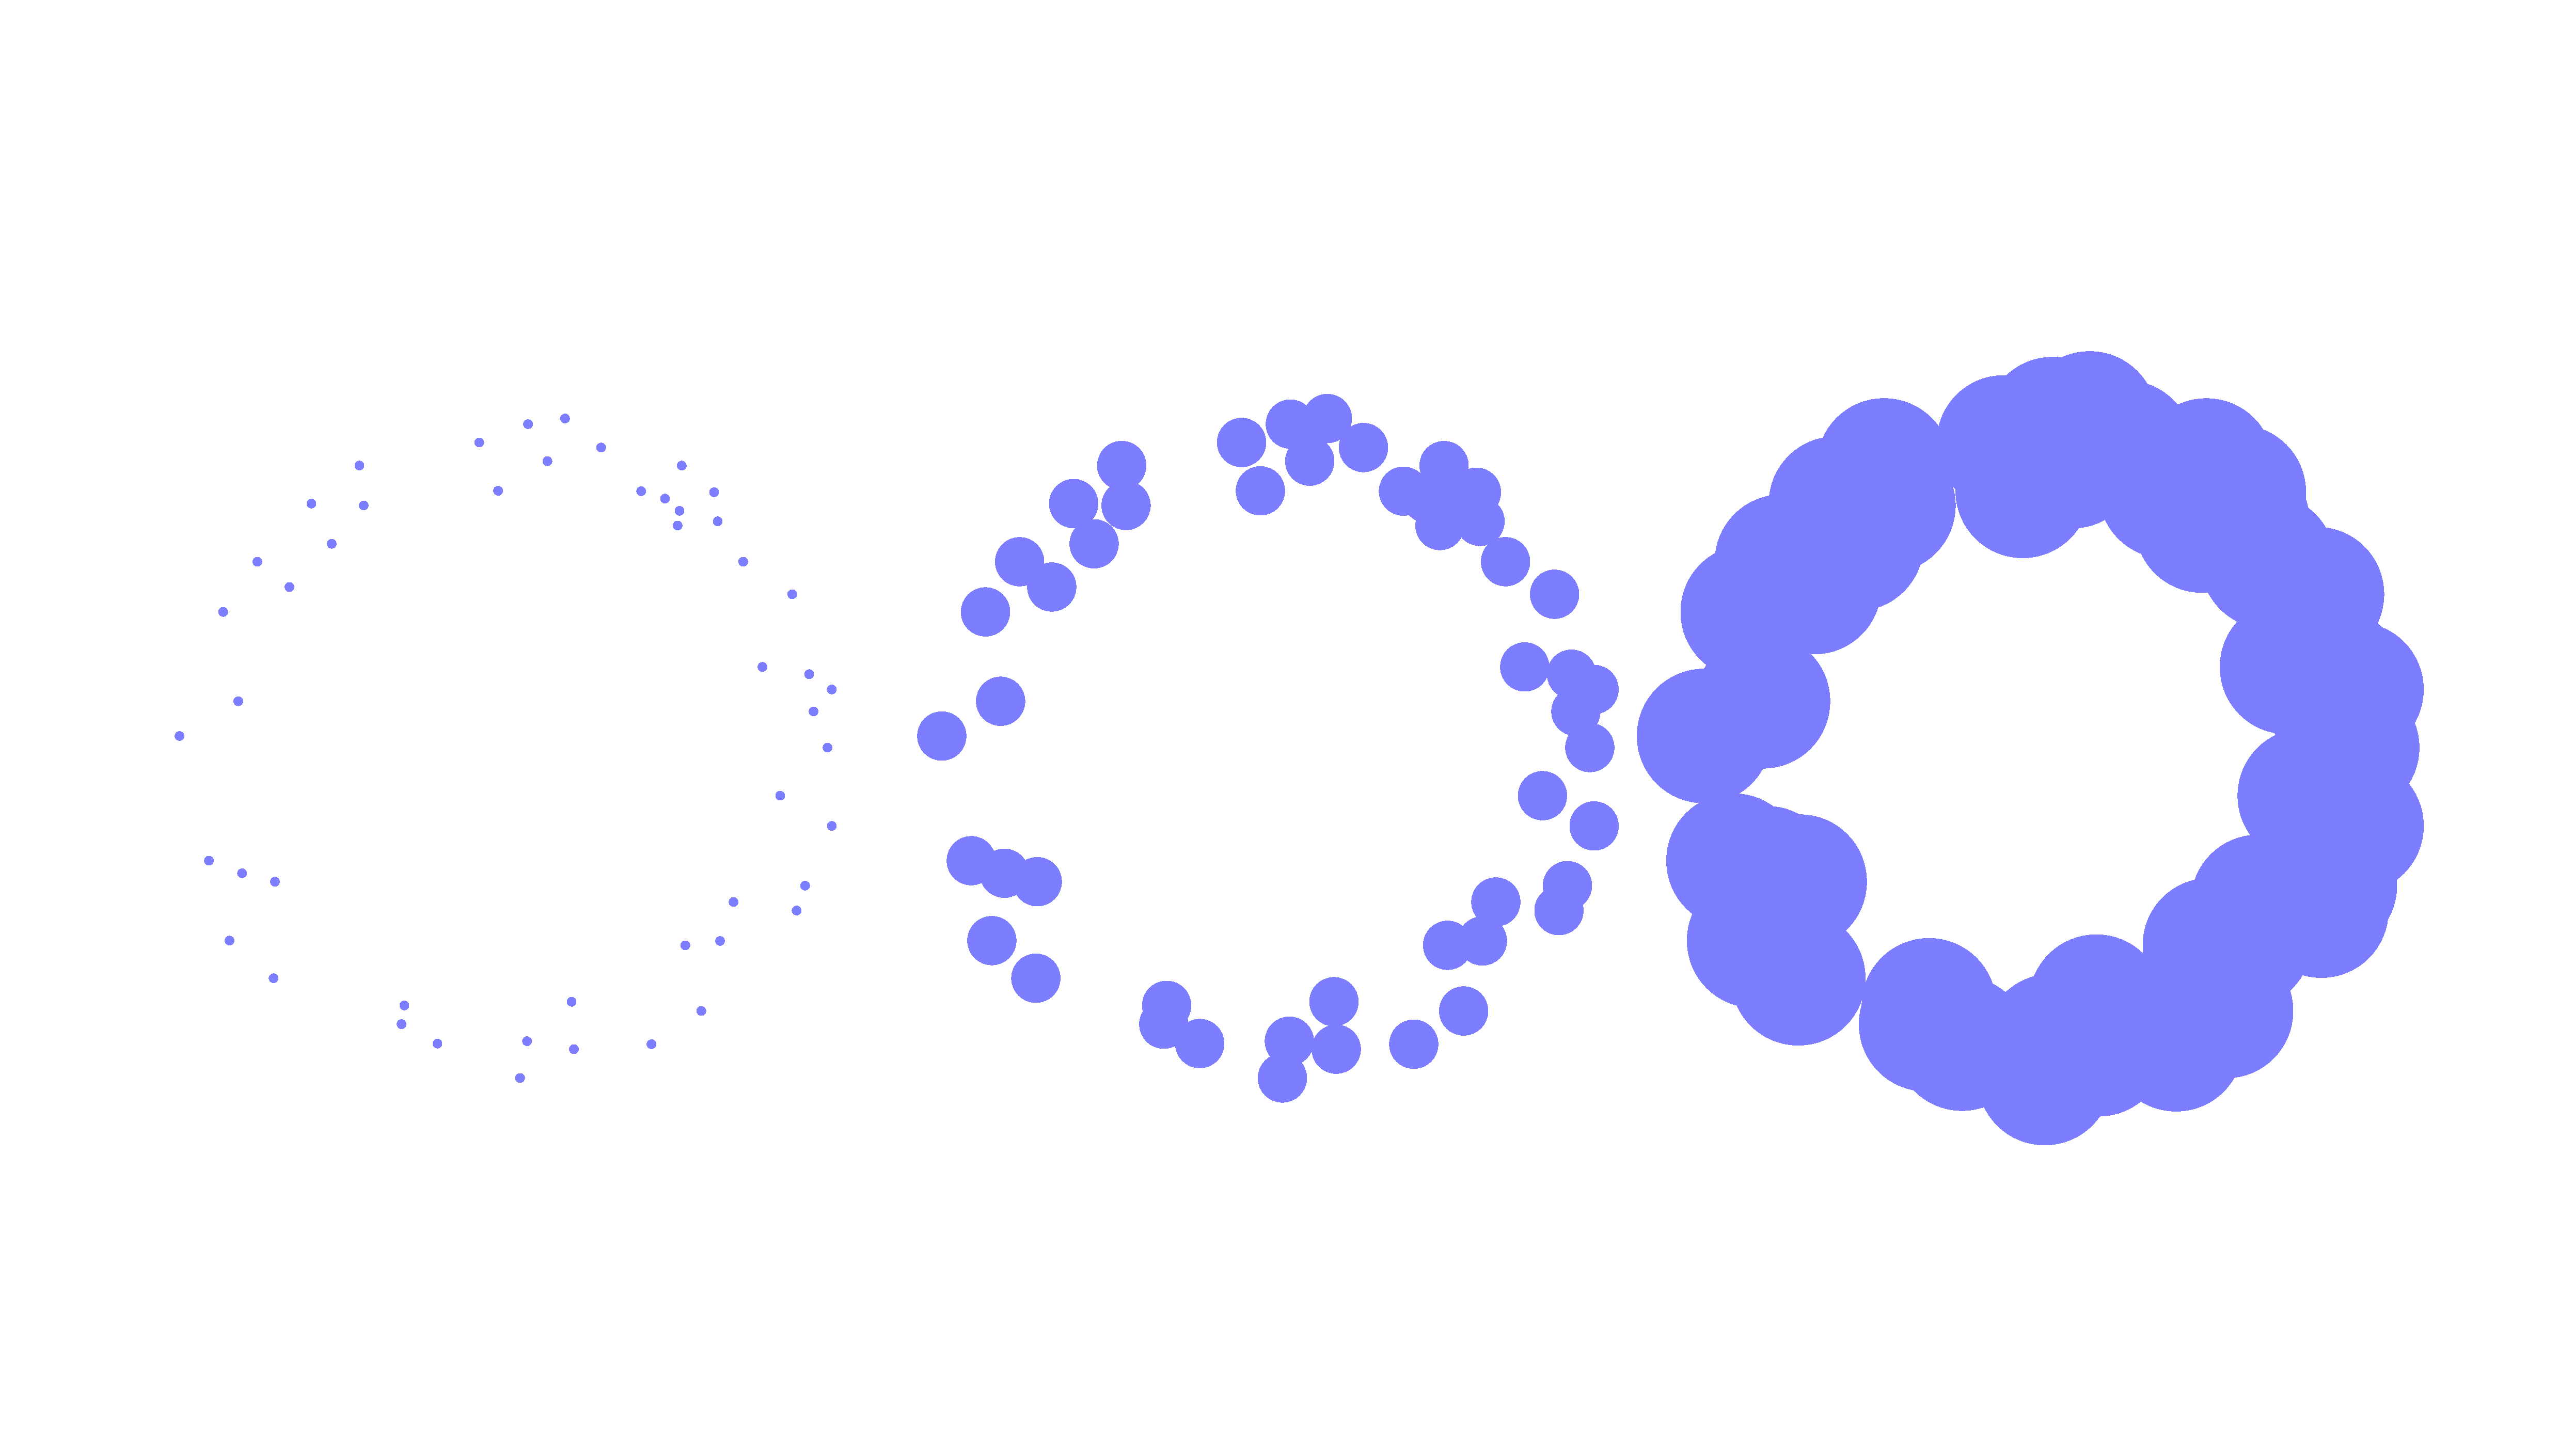
\includegraphics[width=.7\paperwidth]{gfx/statistical_circle_comparison.pdf}
    \caption{$\widehat{Y}_\varepsilon$ al variare di $\varepsilon$}
    \label{fig2:circlecomparison}
  \end{center}
\end{figure}

A questo punto abbiamo a che fare con spazi più o meno noti e, per opportune scelte di $\varepsilon$, si possono calcolare i gruppi di omologia $H_0(\widehat{X}_\varepsilon)$ e $H_1(\widehat{Y}_\varepsilon)$ che racchiudono rispettivamente l'informazione sul numero di cluster in \cref{fig2:clusters} e di loop in \cref{fig2:circle}.

Tuttavia in entrambi questi casi c'è bisogno di selezionare un parametro di scala $\varepsilon$ per cui $\widehat{X}_\varepsilon$ contenga esattamente le informazioni che vogliamo trovare, e questa scelta non sempre è evidente. Ad esempio potrebbe succedere che i dati sono in dimensione talmente alta che non è possibile visualizzarli, oppure proprietà che sono evidenti ad una certa scala scompaiono al variare di $\varepsilon$, mentre ne compaiono di nuove. Quindi siamo alla ricerca di metodi che consentano non solo di dedurre informazioni sulla forma dei dati senza doversi preoccupare della selezione di una scala, ma che riescano anche a mettere in relazione le variazioni di queste proprietà al variare della scala di riferimento. L'insieme delle tecniche che consentono di fare questo e molto altro vanno sotto il nome di Topological Data Analysis (TDA).

Lo sviluppo della TDA è stato iniziato da Carlsson et al. nel 2009 in \cite{Carlsson2009}, con l'obiettivo di riuscire a ricavare a partire da un insieme di dati informazioni \emph{qualitative}, \emph{indipendenti dalla scelta di coordinate} e prediligendo una visione d'insieme. Vi sono stati molti progressi sia nella teoria sia nell'applicazione, ad esempio nello sviluppo della teoria della persistenza multidimensionale \cite{Cerri2013,Carlsson2009a,Adcock2012,Carlsson2009b}, della fondazione categorica della persistenza
\cite{Curry}, dell'utilizzo della persistenza nell'inferenza statistica \cite{Bubenik2015,Kwitt2015}, e la ricerca è tuttora in corso.

Lo strumento principale della TDA è la persistenza omologica, cioé l'assegnazione ad uno spazio metrico finito di una filtrazione di spazi vettoriali $\{V_r\}_{r\in\R}$ in cui gli spazi vettoriali $V_r$ e le mappe fra essi $V_r\to V_s$ per $r<s$ contengano informazioni sulla \emph{forma} dello spazio in esame.

In particolare, gli spazi vettoriali $V_r$ sono gruppi di omologia (e quindi saranno in dicati con $H_q(X_r)$) e il parametro $r$ in genere è preso in $\R^+$ perché identifica una scala di riferimento. Questi gruppi di omologia persistenti vengono visualizzati mediante codici a barre persistenti (\cref{fig:typicalbarcode}), dove ogni linea traccia l'evoluzione di una singola \emph{feature} topologica e la lunghezza ne è la durata.

\begin{figure}[h]
  \begin{center}
    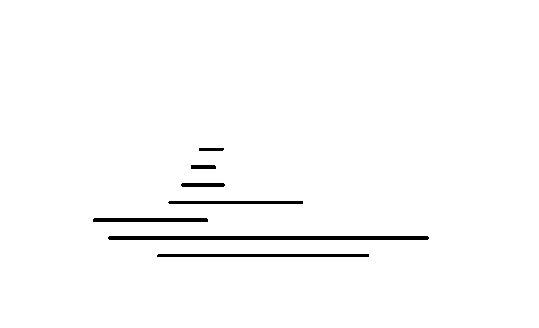
\includegraphics[width=.7\paperwidth]{gfx/barcodes_multiple.pdf}
    \caption{Esempio di codice a barre persistente}
    \label{fig:typicalbarcode}
  \end{center}
\end{figure}

La proprietà fondamentale dei gruppi di omologia persistenti è che essi tengono traccia del legame che vi è fra le proprietà topologiche a diverse scale.

\begin{figure}[ht]
  \begin{center}
    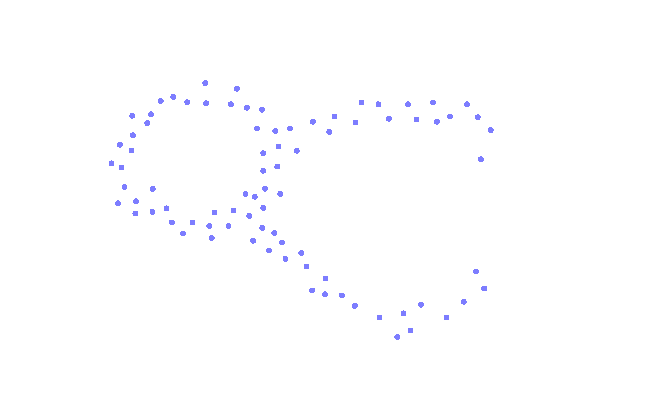
\includegraphics{gfx/double_circle_small.pdf}
    \caption{Un doppio anello}
    \label{fig2:doublecircle}
  \end{center}
\end{figure}

Si consideri ad esempio la nube di punti in \cref{fig2:doublecircle}. Al variare di $r$ compaiono due loop come mostrato in \cref{fig2:doublecirclecomparison}.

\begin{figure}[ht]
  \begin{center}
    \begin{subfigure}[b]{.4\textwidth}
      
\includegraphics[width=\textwidth]{gfx/double_circle_medium.pdf}
      \caption{$\widehat{X}_{r_1}$}
    \end{subfigure}
    \begin{subfigure}[b]{.4\textwidth}
      
\includegraphics[width=\textwidth]{gfx/double_circle_fat.pdf}
      \caption{$\widehat{X}_{r_2}$}
    \end{subfigure}
    \caption{Variazione delle proprietà di $\widehat{X}_r$}  \label{fig2:doublecirclecomparison}
  \end{center}
\end{figure}

 La presenza dei due loop è rappresentata dall'omologia persistente dal fatto che $H_1(\widehat{X}_{r_1})$ e $H_1(\widehat{X}_{r_2})$ hanno entrambi dimensione 1. Tuttavia, l'omologia persistente consente anche di distinguere i due loop. Infatti, poiché $r_1<r_2$ l'omologia persistente viene con una mappa $\psi:H_1(\widehat{X}_{r_1})\to H_1(\widehat{X}_{r_2})$ e il fatto che i due loop sono distinti lo si deduce dal fatto che $\psi=0$.

 Questa proprietà dell'omologia persistente, dettà \emph{funtorialità}, è l'elemento essenziale che rende queste tecniche estremamente utili nelle applicazioni.

 L'altra proprietà fondamentale dell'omologia persistente è enunciata nel \Cref{thm:persistentdecomposition} che garantisce che ogni gruppo di omologia persistente associato ad uno spazio metrico finito può essere rappresentato con un numero finito (idealmente piccolo) di parametri. Questo fatto consente di visualizzare con pochi parametri un insieme di dati potenzialmente complesso, inoltre lo spazio di questi parametri può essere reso uno spazio metrico completo (come in \cite{Kwitt2015}), aprendo spazio all'utilizzo di tecniche di statistica e machine learning.

%************************************************
\chapter{Esempi e applicazioni}\label{cap:esempi}
%************************************************

In questo capitolo mostreremo alcuni esempi con dati sintetici che mostrano il tipo di visualizzazione che si riesce ad ottenere utilizzando l'omologia persistente, poi vedremo come la TDA è stata usata in diversi studi per ricostruire la struttura di un insieme di \emph{patch} ad alto contrasto estratte da immagini naturali.

\section{Esempi in basse dimensioni}

Come primi esempi mostriamo in \cref{fig:examplecirclesbarcodes} i codici a barre persistenti rispettivamente di un cerchio nel piano e di due cerchi nel piano.

\begin{figure}[h]
  \caption{Esempi di codici a barre persistenti}
  \label{fig:examplecirclesbarcodes}
  \centering
  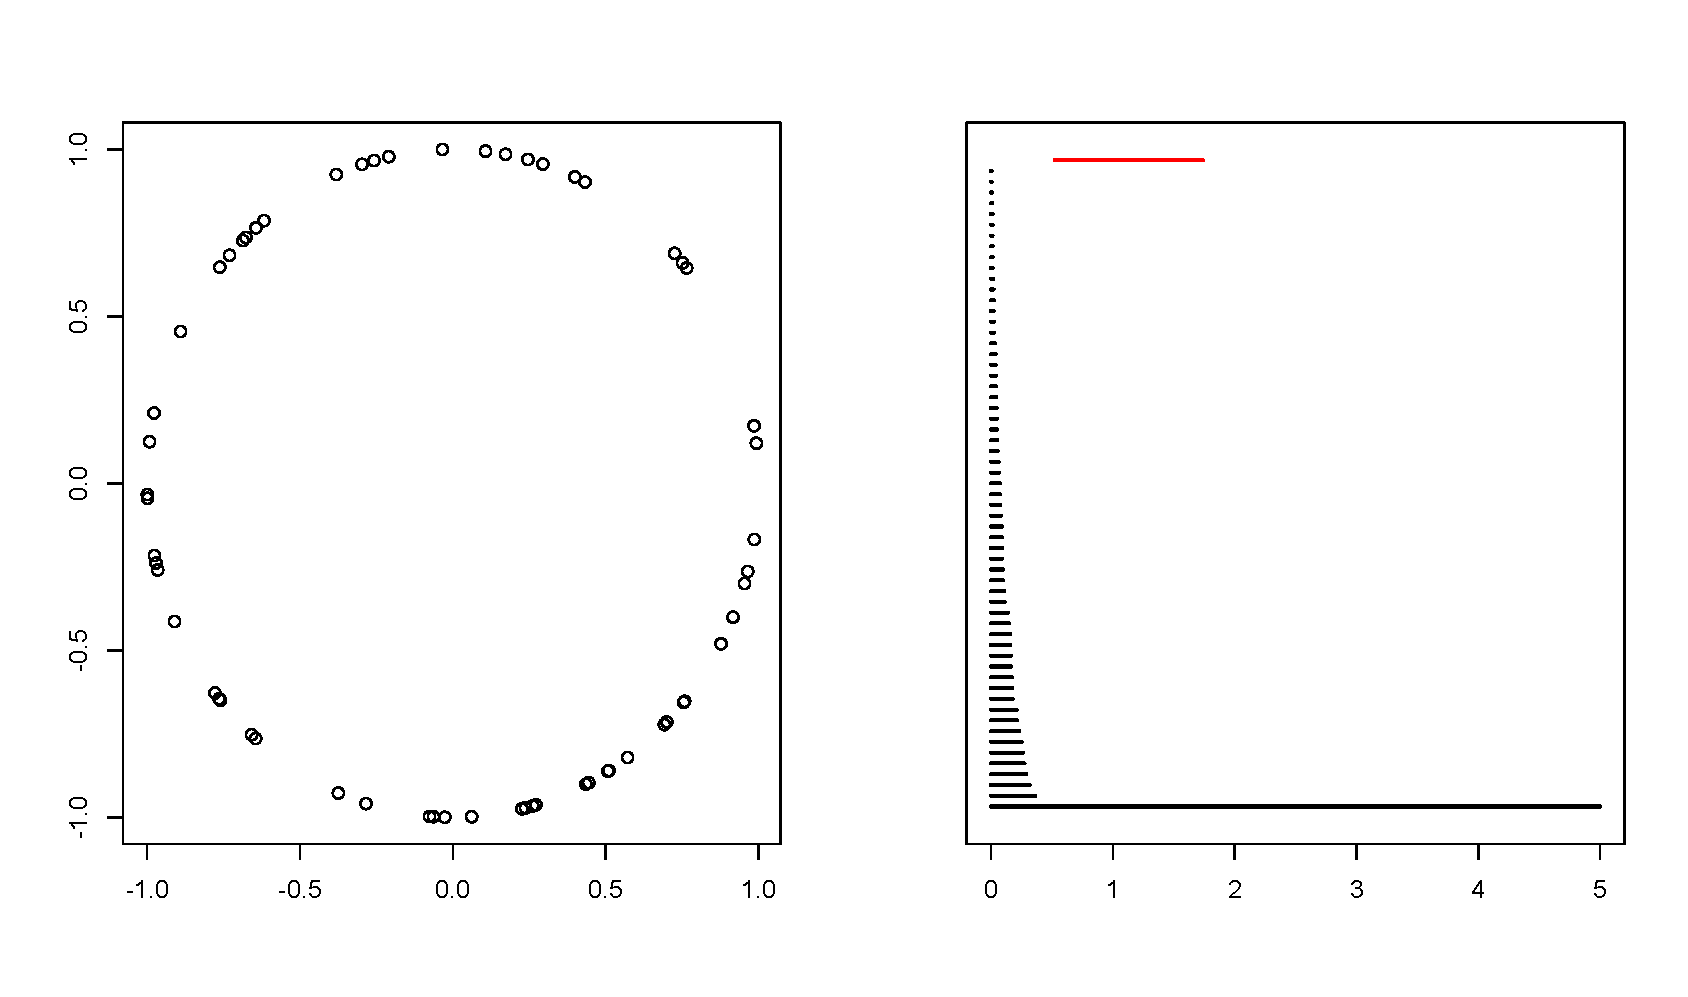
\includegraphics[width=.8\linewidth]{gfx/circle_persistence.pdf}
  \subcaption{Estrazione casuale da un singolo cerchio}
  \centering
  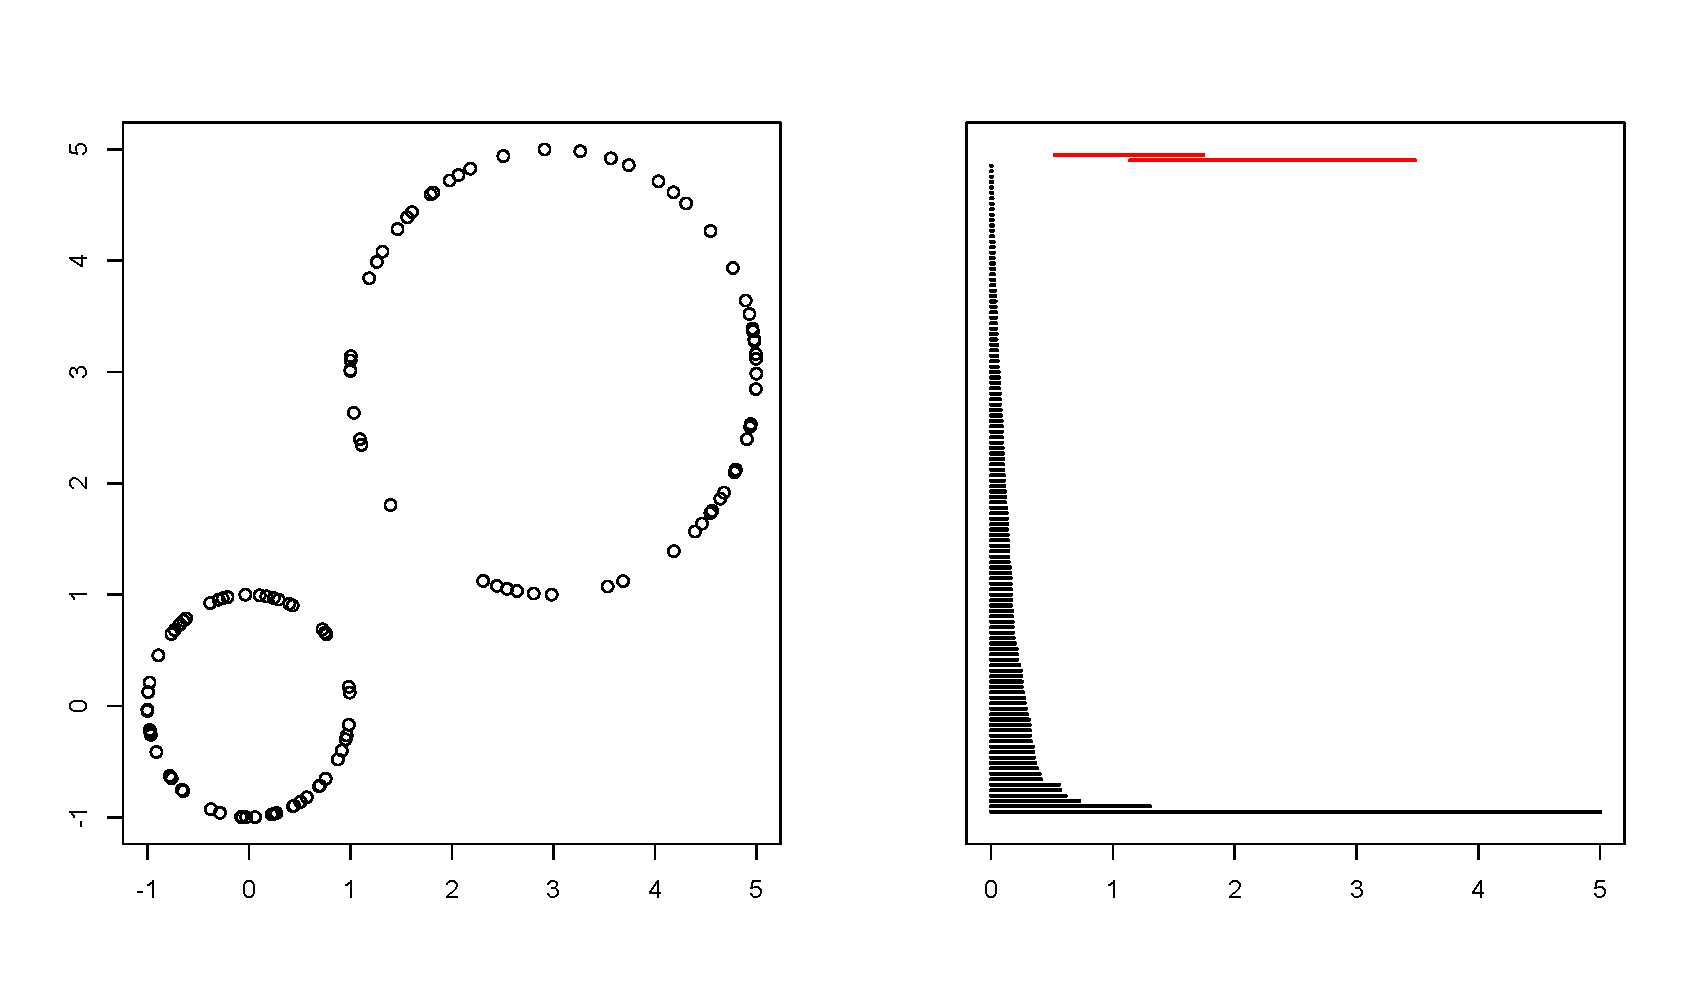
\includegraphics[width=.8\linewidth]{gfx/two_circles.pdf}
  \subcaption{Estrazione casuale da due cerchi}
\end{figure}

Anche in questi casi banali è possibile osservare come la diversa distribuzione dei punti sui cerchi causa interssanti artefatti, come si può osservare dall'omologia persistente 0-dimensionale nel caso dei due cerchi, in cui la presenza di due componenti connesse non è così marcatamente evidente dal codice a barre persistente.


\section{Struttura di un insieme di immagini}

In questa sezione ripercorreremo lo studio omologico di un insieme di immagini costruito da
Lee, Pedersen e Mumford in \cite{Lee2003} e analizzato in \cite{Carlsson2008} e \cite{DeSilva2004}.

L'insieme di dati è composto da immagini in bianco e nero, catturate mediante una fotocamera digitale, e si può pensare a ciascuna di queste immagini come a un vettore di pixel in uno spazio vettoriale di dimensione estremamente alta, e dove la coordinata corrispondente a un certo pixel è il valore nella scala di grigi di quel pixel.

\begin{figure}[ht]
  \begin{center}
    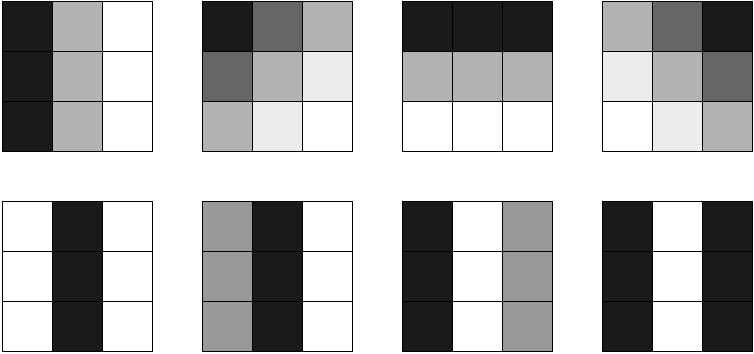
\includegraphics[width=.8\linewidth]{gfx/example_patches.pdf}
    \caption{Esempi di patch $3\times 3$ ad alto contrasto}
    \label{fig:examplepatches}
  \end{center}
\end{figure}

Poiché la dimensione di questo problema è estremamente elevate è impossibile pensare di analizzare direttamente questo insieme, tuttavia si può studiare il problema di dimensione più ridotta di descrivere la statistica delle piccole patch (blocchi $3\times 3$ estratti dalle immagini) ad alto contrasto, come quelle in \cref{fig:examplepatches}.

Detto $\mathcal{M}$ l'insieme di immagini che si vuole studiare, il procedimento che porta a selezionare le patch su cui viene effettuata l'anlisi è il seguente:
\begin{enumerate}
  \item Da ogni immagine di $\mathcal{M}$ vengono estratte casualmente un numero $L$ elevato di patch $3\times 3$. Tutte queste patch vengono considerate come un sottinsieme $\mathcal{P}_1$ di $\R^9$.
  \item Ogni $x\in\mathcal{P}_1$ viene riscalato in $\tilde{x}$ con $\tilde{x}_i = log(x_i)$.
  \item Per ogni vettore $\tilde{x}$ si calcola il suo contrasto (detto anche $D$-norma) $\normD{\tilde{x}}=\sqrt{\tilde{x}^\mathbf{T}D\tilde{x}}$, dove $D$ è una forma quadratica che tiene conto della differenza di ciascun pixel della patch con quelli adiacenti e definita nel seguente modo: scriviamo $i\sim j$ se i pixel corrispondenti all'$i$-ma e $j$-ma coordinata rispettivamente sono adiacenti, e definiamo
  \begin{equation*}
    \normD{x} = \sqrt{\sum_{i\sim j}(x_i-x_j)^2}.
  \end{equation*}
  \item Si conserva solo il $20\%$ delle patch con $D$-norma più alta.
  \item Si sottrae a ogni $\tilde{x}$ la sua media $\mu(x)=\displaystyle\frac{1}{9}\sum_{i=1}^9\,x_i$, in modo che i nuovi punti $\tilde{y}$ si trovino sull'iperpiano $H\subseteq\R^9$ definito da $\sum_{i=1}^9 x_i =0$.
  \item Si normalizza ciascun vettore dividendolo per la sua $D$-norma.
\end{enumerate}

I dati così elaborati si trovano adesso su un ellissoide $S^7\subseteq\R^9$, indichiamo con $\widetilde{\mathcal{M}}$ l'insieme delle patch rinormalizzate. Nel caso analizzato in \cite{Lee2003} e \cite{Carlsson2008} l'insieme è costituito da $4.5 \times 10^6$ patch.

Come è stato fatto nella \cref{sec:functionalpersistence} vogliamo filtrare i dati per densità. Questa volta useremo come funzione di densità $d_k$ con $k$ intero positivo, dove $d_k(x)$ è la distanza di $x$ dal $k$-mo punto di $\widetilde{\mathcal{M}}$ più vicino a $x$. Poiché $d_k$ è una misura inversa di densità, siamo interessati a punti che abbiano $d_k$ piccolo. Questo giustifica la seguente definizione.

\begin{definition}
  Dato un intero $k$ e una percentuale $p$, definiamo il sottinsieme $X(k,p)\subseteq\widetilde{\mathcal{M}}$ come il $p\%$ più piccolo secondo $d_k$.
\end{definition}

\begin{figure}[ht]
  \begin{center}
    \begin{subfigure}[b]{.4\textwidth}
      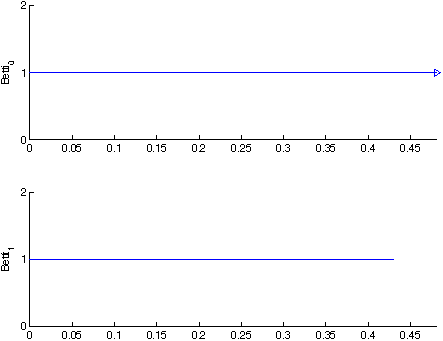
\includegraphics[width=\textwidth]{gfx/image_patches_k300.pdf}
      \caption{$X(300,30)$}\label{fig:k300persistence}
    \end{subfigure}
    \begin{subfigure}[b]{.4\textwidth}
      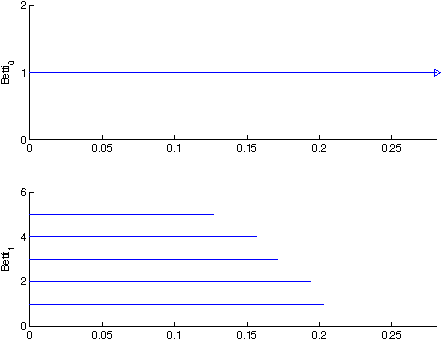
\includegraphics[width=\textwidth]{gfx/image_patches_k15.pdf}
      \caption{$X(15,30)$}\label{fig:k15persistence}
    \end{subfigure}
    \caption{Omologia persistente di $X(k,p)$}
  \end{center}
\end{figure}

A questo punto possiamo studiare al variare dei parametri $k$ e $p$ le proprietà topologiche di $X(k,p)$. Per $k$ grande i dati si dispongono essenzialmente in cerchio, come mostrato dal diagramma di persistenza \cref{fig:k300persistence} tratto da \cite{Carlsson2008}.

% \begin{figure}[ht]
%   \begin{center}
%     \begin{subfigure}
%       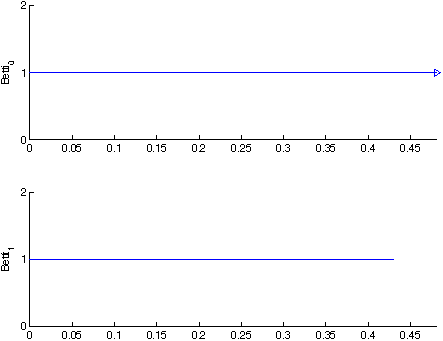
\includegraphics[width=.4\linewidth]{gfx/image_patches_k300.pdf}
%       \subcaption{$X(300,30)$}
%       \label{fig:k3001persistence}
%     \end{subfigure}
%     \begin{subfigure}
%       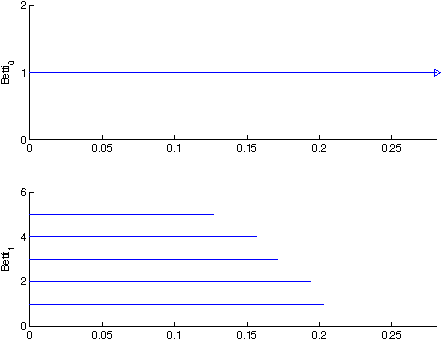
\includegraphics[width=.4\linewidth]{gfx/image_patches_k15.pdf}
%       \subcaption{$X(15,30)$}
%       \label{fig:k15persistence}
%     \end{subfigure}
%   \end{center}
% \end{figure}

\begin{figure}[ht]
  \begin{center}
    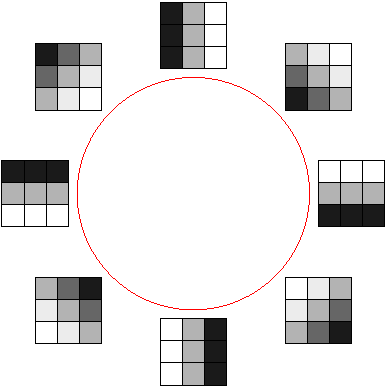
\includegraphics[width=.4\linewidth]{gfx/primarycircle_labels.pdf}
    \caption{Le patch sul cerchio primario}
    \label{fig:primarycircle}
  \end{center}
\end{figure}

In \cite{Carlsson2008} e \cite{DeSilva2004} viene mostrato come sia possibile parametrizzare i dati così selezionati in un cerchio, detto primario. In \cref{fig:primarycircle} lo vediamo rappresentato insieme alle patch che lo compongono.

Se scegliamo un parametro $k$ più piccolo (e quindi selezioniamo punti più densi) vengono scoperte nuove strutture, come si vede dall'omologia persistente di $X(15,30)$ in \cref{fig:k15persistence} (presa da \cite{Carlsson2008}).

% \begin{figure}[ht]
%   \begin{center}
%     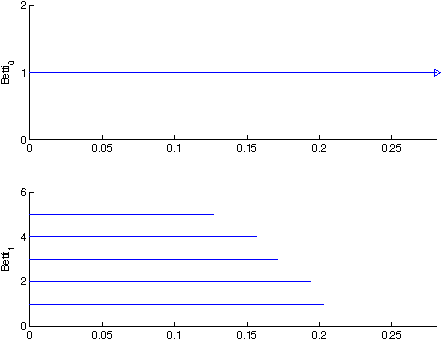
\includegraphics[width=.8\linewidth]{gfx/image_patches_k15.pdf}
%     \caption{L'omologia persistente di $X(15,30)$}
%     \label{fig:k15persistence}
%   \end{center}
% \end{figure}

\begin{figure}[ht]
  \begin{center}
    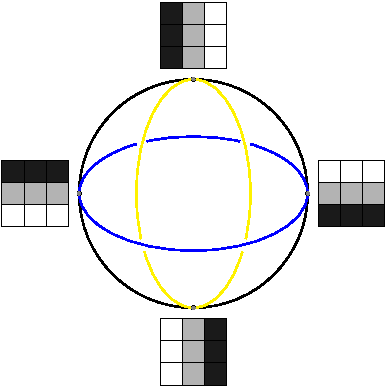
\includegraphics[width=.4\linewidth]{gfx/patches_shape_labels.pdf}
    \caption{La struttura a tre cerchi $C_3$}
    \label{fig:patchshape}
  \end{center}
\end{figure}

Vi sono diversi spazi topologici che hanno questa omologia, e cioé connessi con primo numero di Betti $\beta_1=5$, ad esempio lo spazio mostrato in \cref{fig:patchshape}. In \cite{Carlsson2008} viene data una parametrizzazione dei dati mediante uno spazio di polinomi, e con questi è possibile vedere che la forma rappresentate in \cref{fig:patchshape} è effettivamente corretta.

Possiamo anche visualizzare le patch corrispondenti ai due nuovi cerchi (detti secondari), in \cref{fig:secondarycircle}

\begin{figure}[ht]
  \begin{center}
    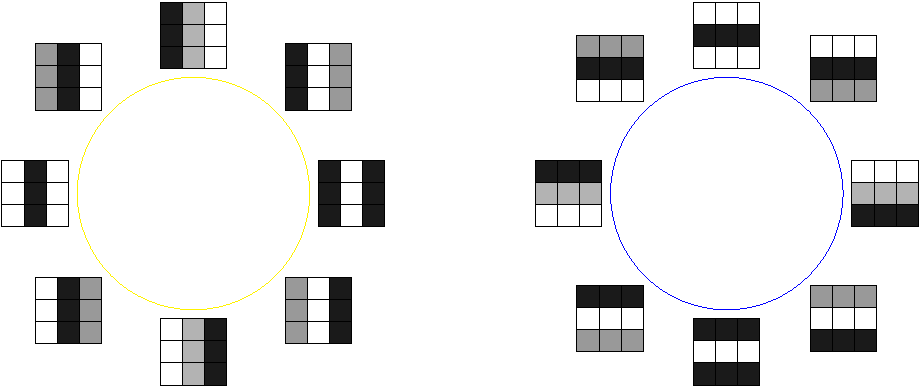
\includegraphics[width=.8\linewidth]{gfx/secondarycircles.pdf}
    \caption{Le patch sui cerchi secondari}
    \label{fig:secondarycircle}
  \end{center}
\end{figure}

Infine, sappiamo da \cite{Carlsson2008} che $X(15,30)$ è contenuto in un insieme di patch che forma una bottiglia di Klein. In \cref{fig:kleinpatch} vediamo come si dispongono i cerchi principali e secondari sulla bottoglia di Klein e come variano le patch.

\begin{figure}[ht]
  \begin{center}
    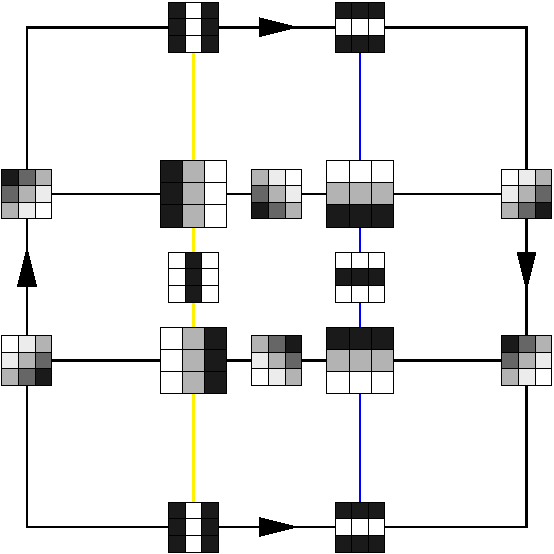
\includegraphics[width=.6\linewidth]{gfx/kleinpatches.pdf}
    \caption{Immersione di $C_3$ nella bottiglia di Klein}
    \label{fig:kleinpatch}
  \end{center}
\end{figure}

% ********************************************************************
% Backmatter
%*******************************************************
%********************************************************************
% Other Stuff in the Back
%*******************************************************
\cleardoublepage%********************************************************************
% Bibliography
%*******************************************************
% work-around to have small caps also here in the headline
\manualmark
\markboth{\spacedlowsmallcaps{\bibname}}{\spacedlowsmallcaps{\bibname}} % work-around to have small caps also
%\phantomsection 
\refstepcounter{dummy}
\addtocontents{toc}{\protect\vspace{\beforebibskip}} % to have the bib a bit from the rest in the toc
\addcontentsline{toc}{chapter}{\tocEntry{\bibname}}
\bibliographystyle{acm}
\label{app:bibliography} 
\bibliography{Bibliography}

%\cleardoublepage\pagestyle{empty}

\hfill

\vfill


\pdfbookmark[0]{Colophon}{colophon}
\section*{Colophon}
This document was typeset using the typographical look-and-feel \texttt{classicthesis} developed by Andr\'e Miede. 
The style was inspired by Robert Bringhurst's seminal book on typography ``\emph{The Elements of Typographic Style}''. 
\texttt{classicthesis} is available for both \LaTeX\ and \mLyX: 
\begin{center}
\url{http://code.google.com/p/classicthesis/}
\end{center}
Happy users of \texttt{classicthesis} usually send a real postcard to the author, a collection of postcards received so far is featured here: 
\begin{center}
\url{http://postcards.miede.de/}
\end{center}
 
\bigskip

\noindent\finalVersionString

%Hermann Zapf's \emph{Palatino} and \emph{Euler} type faces (Type~1 PostScript fonts \emph{URW
%Palladio L} and \emph{FPL}) are used. The ``typewriter'' text is typeset in \emph{Bera Mono}, 
%originally developed by Bitstream, Inc. as ``Bitstream Vera''. (Type~1 PostScript fonts were made 
%available by Malte Rosenau and
%Ulrich Dirr.)

%\paragraph{note:} The custom size of the textblock was calculated
%using the directions given by Mr. Bringhurst (pages 26--29 and
%175/176). 10~pt Palatino needs  133.21~pt for the string
%``abcdefghijklmnopqrstuvwxyz''. This yields a good line length between
%24--26~pc (288--312~pt). Using a ``\emph{double square textblock}''
%with a 1:2 ratio this results in a textblock of 312:624~pt (which
%includes the headline in this design). A good alternative would be the
%``\emph{golden section textblock}'' with a ratio of 1:1.62, here
%312:505.44~pt. For comparison, \texttt{DIV9} of the \texttt{typearea}
%package results in a line length of 389~pt (32.4~pc), which is by far
%too long. However, this information will only be of interest for
%hardcore pseudo-typographers like me.%
%
%To make your own calculations, use the following commands and look up
%the corresponding lengths in the book:
%\begin{verbatim}
%    \settowidth{\abcd}{abcdefghijklmnopqrstuvwxyz}
%    \the\abcd\ % prints the value of the length
%\end{verbatim}
%Please see the file \texttt{classicthesis.sty} for some precalculated 
%values for Palatino and Minion.
%
%    \settowidth{\abcd}{abcdefghijklmnopqrstuvwxyz}
%    \the\abcd\ % prints the value of the length





%\cleardoublepage%*******************************************************
% Declaration
%*******************************************************
\refstepcounter{dummy}
\pdfbookmark[0]{Declaration}{declaration}
\chapter*{Declaration}
\thispagestyle{empty}
Put your declaration here.
\bigskip
 
\noindent\textit{\myLocation, \myTime}

\smallskip

\begin{flushright}
    \begin{tabular}{m{5cm}}
        \\ \hline
        \centering\myName \\
    \end{tabular}
\end{flushright}

% ********************************************************************
% Game Over: Restore, Restart, or Quit?
%*******************************************************
\end{document}
% ********************************************************************
